
\documentclass[5p,times,numbers]{elsarticle}

\usepackage[utf8]{inputenc}
\usepackage[T1]{fontenc}
\usepackage{newunicodechar}
\newunicodechar{́}{\'{}}

\newunicodechar{∆}{\Delta}

\newcommand{\pathtoken}{\mbox{\texttt{\_\_PAT\_<token>\_\_}}}

\usepackage{graphicx}
\usepackage{amssymb}
\usepackage{amsmath}
\usepackage{booktabs}
\usepackage{siunitx}
\usepackage{xcolor}
\usepackage{comment}
\usepackage{xurl}
\usepackage[hidelinks]{hyperref}
\usepackage{microtype}
\usepackage{placeins}
\usepackage[switch]{lineno}
\setlength{\emergencystretch}{3em}


\graphicspath{{figures/}}

\biboptions{numbers,sort&compress}

\begin{document}

\begin{frontmatter}


\title{Existing Multi-Material FFF Printers Are Sufficient For (Near) Arbitrary Coloration}

\begin{abstract}
Color 3D printing is often treated as a hardware problem: producing more colors requires more independently addressable materials, active color mixing, specialized feedstock, or color-aware slicing software. Here we show that existing multi-material fused filament fabrication (FFF) printers can approach near-arbitrary coloration by using layer geometry rather than additional color-mixing hardware. LayerLoom encodes color as repeated vertical sequences of standard filaments by decomposing colored 3MF or GLB models into interleaved Z-bands whose layer sequences encode discrete layer-fraction recipes. Because these schedules are carried by ordinary mesh geometry, downstream slicers process the result as a conventional multi-object, multi-material print rather than as a custom color-mixing operation.

We enumerate valid layer-fraction recipes under weave-height, run-length, and endpoint constraints and evaluate the resulting prints using calibrated CIE \(L^*a^*b^*\)/CIEDE2000 image measurements. With three CMY filaments, the full printed gamut produced 51 distinguishable clusters from 55 measured regions at \(\Delta E_{00}<2\). Expanded secondary and neutral endpoints produced 393 distinguishable clusters from 1,210 measured regions. Print-time and material benchmarks show that woven colors impose the least overhead when they reuse filaments already active on the same layers, while larger increases occur when a workflow introduces additional physical filament channels. These results show that layer-wise material order can be encoded as portable 3MF geometry, allowing ordinary multi-material FFF printers to produce more distinguishable printed colors without custom extrusion hardware, custom feedstock, modified G-code, or slicer-specific color-mixing tools. LayerLoom is free and open-source.
\end{abstract}


\begin{keyword}
Fused filament fabrication \sep multi-material 3D printing \sep color 3D printing \sep layer weaving \sep 3MF \sep computational fabrication
\end{keyword}

\end{frontmatter}
\linenumbers

\begin{figure*}[!t]
    \centering
    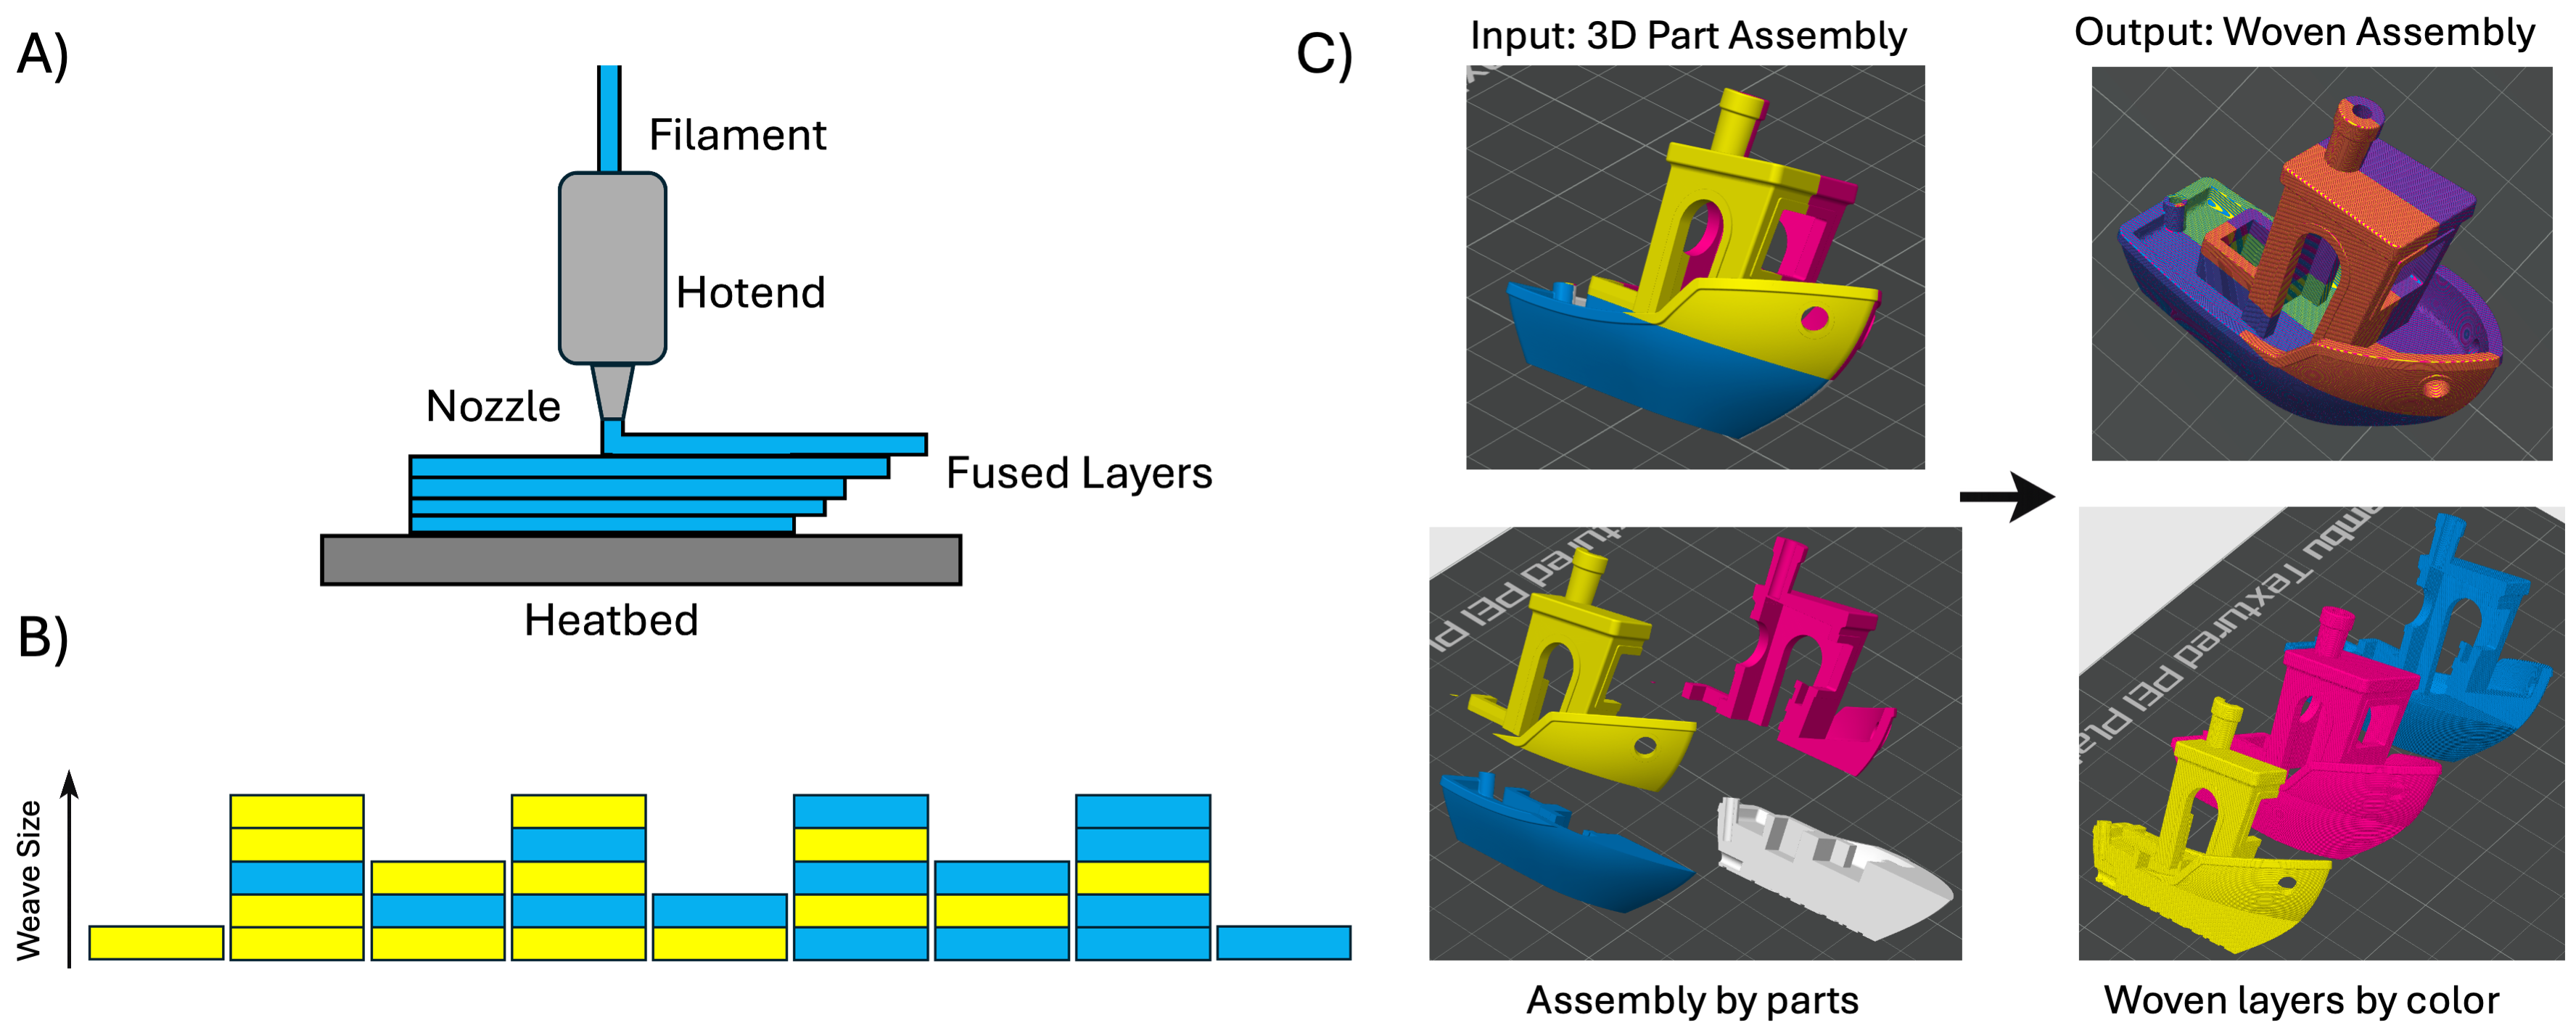
\includegraphics[width=0.95\linewidth]{fig01_layer_weaving_principle.png}
    \par\vspace{3pt}
    \begingroup
    \small
    \setlength{\tabcolsep}{4pt}
    \begin{tabular}{c@{\quad$\longrightarrow$\quad}c@{\quad$\longrightarrow$\quad}c@{\quad$\longrightarrow$\quad}c}
    \textbf{1} Colored input &
    \textbf{2} Separate source-color parts &
    \textbf{3} Cut repeated Z-bands &
    \textbf{4} Regroup by filament
    \end{tabular}
    \endgroup
    \caption{
    \textbf{LayerLoom workflow and layer-weaving principle.} \textbf{A}, filament deposition fuses successive physical layers into FFF geometry. \textbf{B}, a target color is encoded as a repeated stack of colored Z-layers, with weave size setting the vertical repeat period. \textbf{C}, the numbered guide summarizes the geometry workflow: a colored input assembly is separated into source-color parts, cut into repeated Z-bands, and regrouped into filament-specific output objects. The maximum same-color run length limits adjacent layers assigned to a filament.
}
    \label{fig:basic-principle}
\end{figure*}


\section{Introduction}

Low-cost fused filament fabrication (FFF) has made multi-material 3D printing increasingly accessible, but color reproduction in desktop material-extrusion systems remains tied to the number of physical materials a printer can deposit. In most workflows, each loaded filament corresponds to one directly printable color. Expanding the palette therefore usually requires more material channels, color-mixing hardware, specialized feedstock, or printer-architecture-specific software that plans color transitions during slicing.

This creates a practical gap: many users now have multi-material FFF hardware, but still have access to only a small number of printed colors. LayerLoom addresses this gap by treating printed color as a repeated layer sequence rather than as a single material assignment (Fig.~\ref{fig:basic-principle}). Instead of assigning each displayed color to a separate filament, LayerLoom converts colored regions into interleaved Z-bands assigned to the physical filaments already loaded in the printer. A target woven color is represented as a repeating weave pattern: a sequence of filament assignments that encodes a discrete layer-fraction recipe. Because this schedule is stored as ordinary 3MF geometry, the generated model can be processed by standard multi-material slicers while carrying both shape and woven color structure downstream.

This paper makes three contributions. First, it introduces a geometry-level representation for color scheduling in which repeated material sequences are encoded as filament-specific Z-bands inside ordinary 3MF assemblies. Second, it describes an algorithmic workflow for importing colored 3MF or GLB models, enumerating constrained layer-fraction recipes, assigning woven recipes, and reconstructing slicer-ready per-filament geometry. Third, it evaluates the representation using printed color gamuts, calibrated CIE ($L^*a^*b^*$)/CIEDE2000 measurements, application-oriented scientific models, and multi-material print-time benchmarks. The central contribution is a portable geometric encoding that lets existing slicers fabricate expanded-color FFF objects from standard multi-material model files.

\section{Related Work}

Prior approaches to richer 3D printed color can be grouped by where they place the color-generation problem. One route mixes materials during extrusion. Multi-in-one-out nozzles and related dynamic color-mixing systems combine differently colored feedstocks before deposition, but color transitions require the previous mixture to be displaced from the melt zone and nozzle before a new mixture stabilizes. These transitions are not instantaneous and can be difficult to predict when frequent or precise color changes are required \citep{hergel2014clean,song2019colored}. Active mixing systems also introduce process-control challenges, including sensitivity to feed parameters, nozzle behavior, clogging, and uneven mixing \citep{li2019experimental}. A related feedstock route pre-encodes material variation into the filament itself, for example by fabricating programmable or heterogeneous filaments that can be printed using otherwise standard FFF hardware \citep{takahashi2020programmable,ahn2024digital}. These approaches avoid some slicer-side color planning, but shift the color-generation step into custom material preparation.

A second category changes the exposed surface or deposited process rather than the nozzle mixture. Reiner et al. used dual-extrusion FDM to produce two-tone imagery by modifying surface geometry: black and white layers were arranged into offset, gear-tooth-like protrusions so that different amounts of each material remained visible from the outside \citep{reiner2014dualcolor}. Kuipers et al. formalized a related line-based halftoning method by varying the visible widths of alternating black and white lines \citep{kuipers2018hatching}, and Song et al. varied extrusion height to control layered color \citep{song2019colored}. These surface/process methods make their color decision in a visible geometric or toolpath feature, whereas LayerLoom stores a repeated through-thickness schedule in the model.

A third category is slicer-native color mixing. Full Spectrum and Bambu Studio's Color Mixing feature resolve colors through software- or plugin-specific virtual-material planning during slicing and G-code generation \citep{ratdoux2026fullspectrum,bambu2026studio253}. LayerLoom differs by completing color scheduling before slicing and carrying the resulting schedule in conventional mesh geometry; this makes the colored model transferable, provided that the receiving slicer preserves the weave-height Z registration and the object-to-filament mapping.

Appearance-driven and voxel-oriented 3D printing places color and appearance inside the object volume. Volumetric color and contoning methods can improve tone, contrast, and detail by distributing material through translucent media \citep{babaei2017color,brunton2016pushing}. Related work on reproducing subsurface scattering shows that perceived appearance depends on how light interacts with internal material distributions, not only on the identity of the outermost surface layer \citep{dong2010fabricating,hasan2010physical,sumin2019geometry,rittig2021neural}. Voxel-level material assignment can also require specialized computational pipelines and high-throughput material streaming \citep{vidimce2013openfab}. Related dithering and voxel-composition methods show similar promise, but highly fragmented material distributions can introduce artifacts or mechanical tradeoffs \citep{cho2003dithering,willmott2023three,morsy2022shape}.

LayerLoom is closest in spirit to passive layered-tone methods, but differs in where the repeated material schedule is represented. Rather than relying on specialized hardware, modified G-code, custom toolpaths, or a slicer-native virtual material model, LayerLoom performs the color-scheduling step before slicing and writes the result as ordinary filament-assigned 3MF geometry. Each woven color is represented by interleaved Z-bands assigned to the physical filaments already loaded in the printer. Once this woven geometry has been generated, downstream software does not need to solve or interpret the color schedule: slicers process the file as a standard multi-part, multi-material object, and the printer executes ordinary filament assignments. Portability is therefore conditional rather than universal: the slicer must retain the generated Z positions at the selected weave height and keep each output object mapped to its intended physical filament.


\section{LayerLoom in Detail}

The terms used in the workflow are defined in Table~\ref{tab:terms}.

\begin{table*}[!t]
\centering
\caption{\textbf{LayerLoom terms used in the workflow.} The maximum token length \(H\) and the physical band height \(h\) are distinct parameters.}
\small
\begin{tabular}{p{0.22\linewidth}p{0.70\linewidth}}
\toprule
Term & Operational definition \\
\midrule
Endpoint filament & One physical filament loaded in the printer and available to the recipe. \\
Stack token & A written sequence of endpoint labels, such as \texttt{cmy} or \texttt{cmymy}, repeated through the Z direction. \\
Layer-fraction recipe & The normalized endpoint counts implied by a token; \texttt{cmy}, \texttt{myc}, and \texttt{ymc} all encode the same 1:1:1 C:M:Y fraction. \\
Maximum weave length \(H\) & The maximum number of physical layers in one repeating stack token. \\
Physical layer height \(h\) & The slicer layer thickness and Z-band height in millimeters. \\
Same-color run length & The longest adjacent run of one endpoint in the repeated token, including its wraparound boundary. \\
Filament-specific output object & The accumulated geometry for one physical filament, such as \texttt{all\_cyan}. \\
\bottomrule
\end{tabular}
\label{tab:terms}
\end{table*}

LayerLoom operates on geometry prior to slicing, using the object, component, and packaging structure defined by the 3MF Core Specification \citep{three_mf_core_1_3}. The implementation accepts colored 3MF files and color-coded GLB meshes, and emits a woven 3MF in which output objects correspond to physical filament assignments. Downstream slicers therefore treat the result as a conventional multi-object, multi-material model.

The workflow can be read as a single transformation. First, a colored input region retains its source color. LayerLoom matches that color to an available palette entry and assigns a stack token, for example \texttt{cmymy}. The model is cut into equal-height Z-bands; successive bands receive the successive letters of the token, repeating from the start after the final letter. Finally, all cyan, magenta, and yellow bands are regrouped into their respective output objects. The resulting 3MF contains ordinary meshes plus the geometry-level color schedule shown in Fig.~\ref{fig:basic-principle}.

The available woven colors are defined by the loaded endpoint filaments and a small set of pattern constraints: maximum token length \(H\), maximum same-color run length, and the number of distinct filaments permitted in a token. This study uses CMY as the baseline and also tests black, white, light gray, dark neutral gray, orange, violet, and green endpoints.

A reported color recipe is defined by the reduced layer-fraction vector of a valid stack token rather than by every ordering of that token. Thus, \texttt{cmy}, \texttt{myc}, and \texttt{ymc} represent the same 1:1:1 C:M:Y recipe. Recipe counts therefore collapse orderings with identical layer fractions.

For each layer-fraction recipe, LayerLoom selects one canonical written stack token from among valid permutations with the same reduced material fractions. Candidate tokens are ranked by run quality before lexical order: the preferred token minimizes the longest same-color run, minimizes the amount of run length beyond two, favors a larger number of two-layer pairs, favors more alternating runs, and finally uses lexicographic order as a deterministic tie-break. This favors balanced written tokens such as \texttt{cmc} over less evenly distributed alternatives such as \texttt{ccm} when both encode the same material fractions. Run-length constraints are evaluated on the repeated token, including the boundary between the end and beginning of the written token, so a sequence cannot satisfy the rule only by placing repeated colors across the wraparound boundary.

LayerLoom supports several routes for assigning recipes to imported parts. The graphical interface allows manual assignment, which was the default workflow for the examples in this study. Recipes can also be assigned by matching preserved source-color metadata to the nearest available LayerLoom palette entry or by reading stack-token labels embedded in part names or metadata, such as \texttt{\_\_PAT\_cmymy\_\_}. After assignment, LayerLoom performs the color-scheduling step before slicing and writes the result as ordinary filament-assigned 3MF geometry.

LayerLoom cuts each assigned part or colored region into horizontal Z-bands and applies its stack token in order through the model. Bands assigned to the same filament are then merged into one output object, even though they occur at different heights. The resulting 3MF stores both the model shape and the layer-level filament schedule as ordinary mesh geometry, remaining compatible with conventional mesh-based workflows \citep{vidimce2013openfab,willmott2023three}.


\section{LayerLoom Algorithmic Workflow}

LayerLoom converts an input 3MF or GLB into a slicer-ready multi-material 3MF through the following numbered procedure.
\begin{enumerate}
    \item Import and flatten build-reachable source geometry, applying transforms and converting units to millimeters.
    \item Preserve source-color and explicit stack-token metadata when present; otherwise match each source color to the selected palette.
    \item Enumerate valid canonical tokens under the selected endpoint alphabet, maximum token height \(H\), run-length limit, and endpoint-count restriction.
    \item Slice each assigned region into Z-bands of physical height \(h\), then assign band \(k\) to token position \(k \bmod n\).
    \item Accumulate all bands for each endpoint into one filament-specific output object and write a standard multi-object 3MF.
    \item In the receiving slicer, retain the output Z registration at height \(h\) and map every output object to its intended physical filament.
\end{enumerate}

The implementation details below specify the importer, palette enumeration, and geometric clipping used for these steps.

First, the input 3MF is normalized into an internal generic 3MF. LayerLoom reads the 3MF package relationships to identify the root model file, then traverses build items, local component assemblies, and production-extension child model references using \texttt{p:path}. For each build-reachable printable mesh, object and component transforms are composed, unit scales are converted to millimeters, and the transformed vertices are written into a flattened mesh object. Thus, assemblies and repeated instances are converted into editable concrete parts. Part names, source object identifiers, \texttt{source\_hex}, and \texttt{stack\_token} metadata are preserved when available.

GLB inputs are imported into the same representation using their component geometry and color information. Each editable part receives a weave signature, or stack token, either by automatic source-color matching or manual assignment in the graphical interface. If a part name or metadata contains a stack-token tag, such as \texttt{\_\_PAT\_cmymy\_\_}, LayerLoom uses it directly. Token-tagged inputs can therefore be processed headlessly, allowing LayerLoom color assignment and weaving to operate as an automated step in larger modeling workflows.

Palette entries are generated by enumerating valid CMY or expanded CMYKWN/OVG stack sequences under constraints on maximum pattern height, maximum repeated runs, and number of distinct colors. Throughout this manuscript, the two-color rule set denotes \(H \leq 6\), run \(\leq 2\), and at most two distinct endpoints; the normal GUI preset denotes \(H \leq 6\), run \(\leq 3\), and at most three endpoints; and the full rule set denotes \(H \leq 6\), run \(\leq 5\), and at most five endpoints. The 4,647 CMYKWN+OVG theoretical count corresponds to the full rule set using CMY, black, white, one neutral gray, orange, violet, and green. The printed expanded-endpoint measurements are separate from this full theoretical combined palette: the 1,210 measured regions are pooled full-condition printed regions from three-endpoint substitution gamuts.

For weaving, LayerLoom slices each mesh into horizontal Z-bands of physical height \(h\). In the tested workflows, \(h\) was set equal to the slicer layer height. Let \(z_0\) be the minimum Z coordinate across the imported scene. For a mesh \(M\), LayerLoom considers bands
\[
B_k = \{(x,y,z) \in M : z_0 + kh \leq z < z_0 + (k+1)h\}.
\]
Each band index \(k\) is assigned to the corresponding token position \(k \bmod n\), where \(n\) is the length of the part's stack token. Geometry is cut using capped planar mesh clipping; if that fails, LayerLoom falls back to Boolean intersection with a thin slab box. A small vertical tolerance gap of \(10^{-3}\,\mathrm{mm}\) is applied at band boundaries to reduce coincident cap degeneracies. Mesh loading, transformation, clipping, and visualization used trimesh, PyVista, and VTK \citep{trimesh,sullivan2019pyvista,schroeder2006vtk}.

After slicing, all bands assigned to the same final filament token are accumulated into one mesh group, for example \texttt{all\_cyan}, \texttt{all\_magenta}, and \texttt{all\_yellow}. Disconnected shells are allowed inside these grouped objects. The resulting 3MF therefore contains one printable object or assembly per filament color rather than one object per layer band. Object names, part numbers, and metadata encode the intended color assignment for downstream slicers.

The downstream slicer does not need to solve the palette problem or interpret woven color as a special color-mixing operation. It only needs to preserve the generated Z positions, slice at the weave height, and assign the resulting objects to the corresponding physical filaments. LayerLoom woven 3MF outputs were opened and sliced as ordinary multi-object, multi-material models in OrcaSlicer, Bambu Studio, and PrusaSlicer when the slicer layer height matched the weave height. Cura also worked, but required disabling automatic drop-to-plate behavior because that setting moves separated components to the build plate and disrupts the intended Z sequence.

\FloatBarrier





\section{Results}
\subsection{Geometry and Weave Constraints Shape the Accessible Color Space}

Colors attainable by LayerLoom are not uniformly distributed across the CMY gamut.
To determine which colors are reachable under different weaving constraints, we enumerated all valid CMY layer stacks up to a specified maximum stack height, maximum run length of repeated colors, and maximum number of distinct colors.
Each stack was converted into a CMY composition by counting the fraction of cyan, magenta, and yellow layers in the repeating token.
These fractions were then plotted in barycentric coordinates within the CMY ternary triangle (Fig.~\ref{fig:cmy-voronoi}).
This is a nearest-neighbor construction in CMY fraction space, not a perceptual color-difference calculation.
The filled Voronoi regions show how the continuous CMY composition triangle is partitioned among available discrete woven stacks.
Restricting patterns to one- and two-color stacks leaves the triangle interior sparsely represented, whereas allowing three-color stacks and longer patterns adds interior recipes and reduces the size of the nearest-neighbor regions.
Direct CMY printing provides only three directly assigned filament colors.
LayerLoom expands this design space by treating color as a discrete layer-fraction recipe rather than as a one-to-one material assignment (Fig.~\ref{fig:cmy-voronoi}; Table~\ref{tab:palette-family-counts}; Table~S1).
Under the simple rule set \((H \leq 6,\ \mathrm{run} \leq 2,\ \leq 2\ \mathrm{colors})\), CMY produces 30 unique recipes: three pure colors and 27 binary mixtures.
Under the normal rule set \((H \leq 6,\ \mathrm{run} \leq 3,\ \leq 3\ \mathrm{colors})\), CMY produces 55 unique recipes, consisting of three pure colors, 33 binary mixtures, and 19 ternary mixtures.
An extended written-token rule set \((H \leq 7,\ \mathrm{run} \leq 6,\ \leq 3\ \mathrm{colors})\) produces 88 unique CMY layer-fraction recipes.
These counts collapse redundant orderings with identical layer fractions, so permutations such as \texttt{cym}, \texttt{cmy}, and \texttt{mcy} are counted as one expected color recipe.
\begin{table*}[!t]
\centering
\caption{\textbf{Theoretical expansion of expected color recipes under LayerLoom palette rules.}
Counts represent unique layer-fraction recipes after collapsing redundant orderings with identical color fractions.
They are design-space counts, not counts of experimentally resolved color states.
Here, \(N\) denotes a neutral gray endpoint.}
\small
\begin{tabular}{lrrrr}
\toprule
Palette family & Simple $(6,2,2)$ & Normal $(6,3,3)$ & Full $(6,5,5)$ & Unrestricted 6-layer \\
\midrule
K/W only & 11 & 13 & 13 & 13 \\
K/W/N & 30 & 55 & 55 & 55 \\
CMY & 30 & 55 & 55 & 55 \\
OVG & 30 & 55 & 55 & 55 \\
CMYKW & 95 & 305 & 386 & 386 \\
CMYKWN & 141 & 551 & 812 & 813 \\
CMY + OVG & 141 & 551 & 812 & 813 \\
CMYKWN + OVG & 333 & 2001 & 4647 & 4731 \\
\bottomrule
\end{tabular}
\label{tab:palette-family-counts}
\end{table*}


\begin{figure*}[!t]

 \centering
    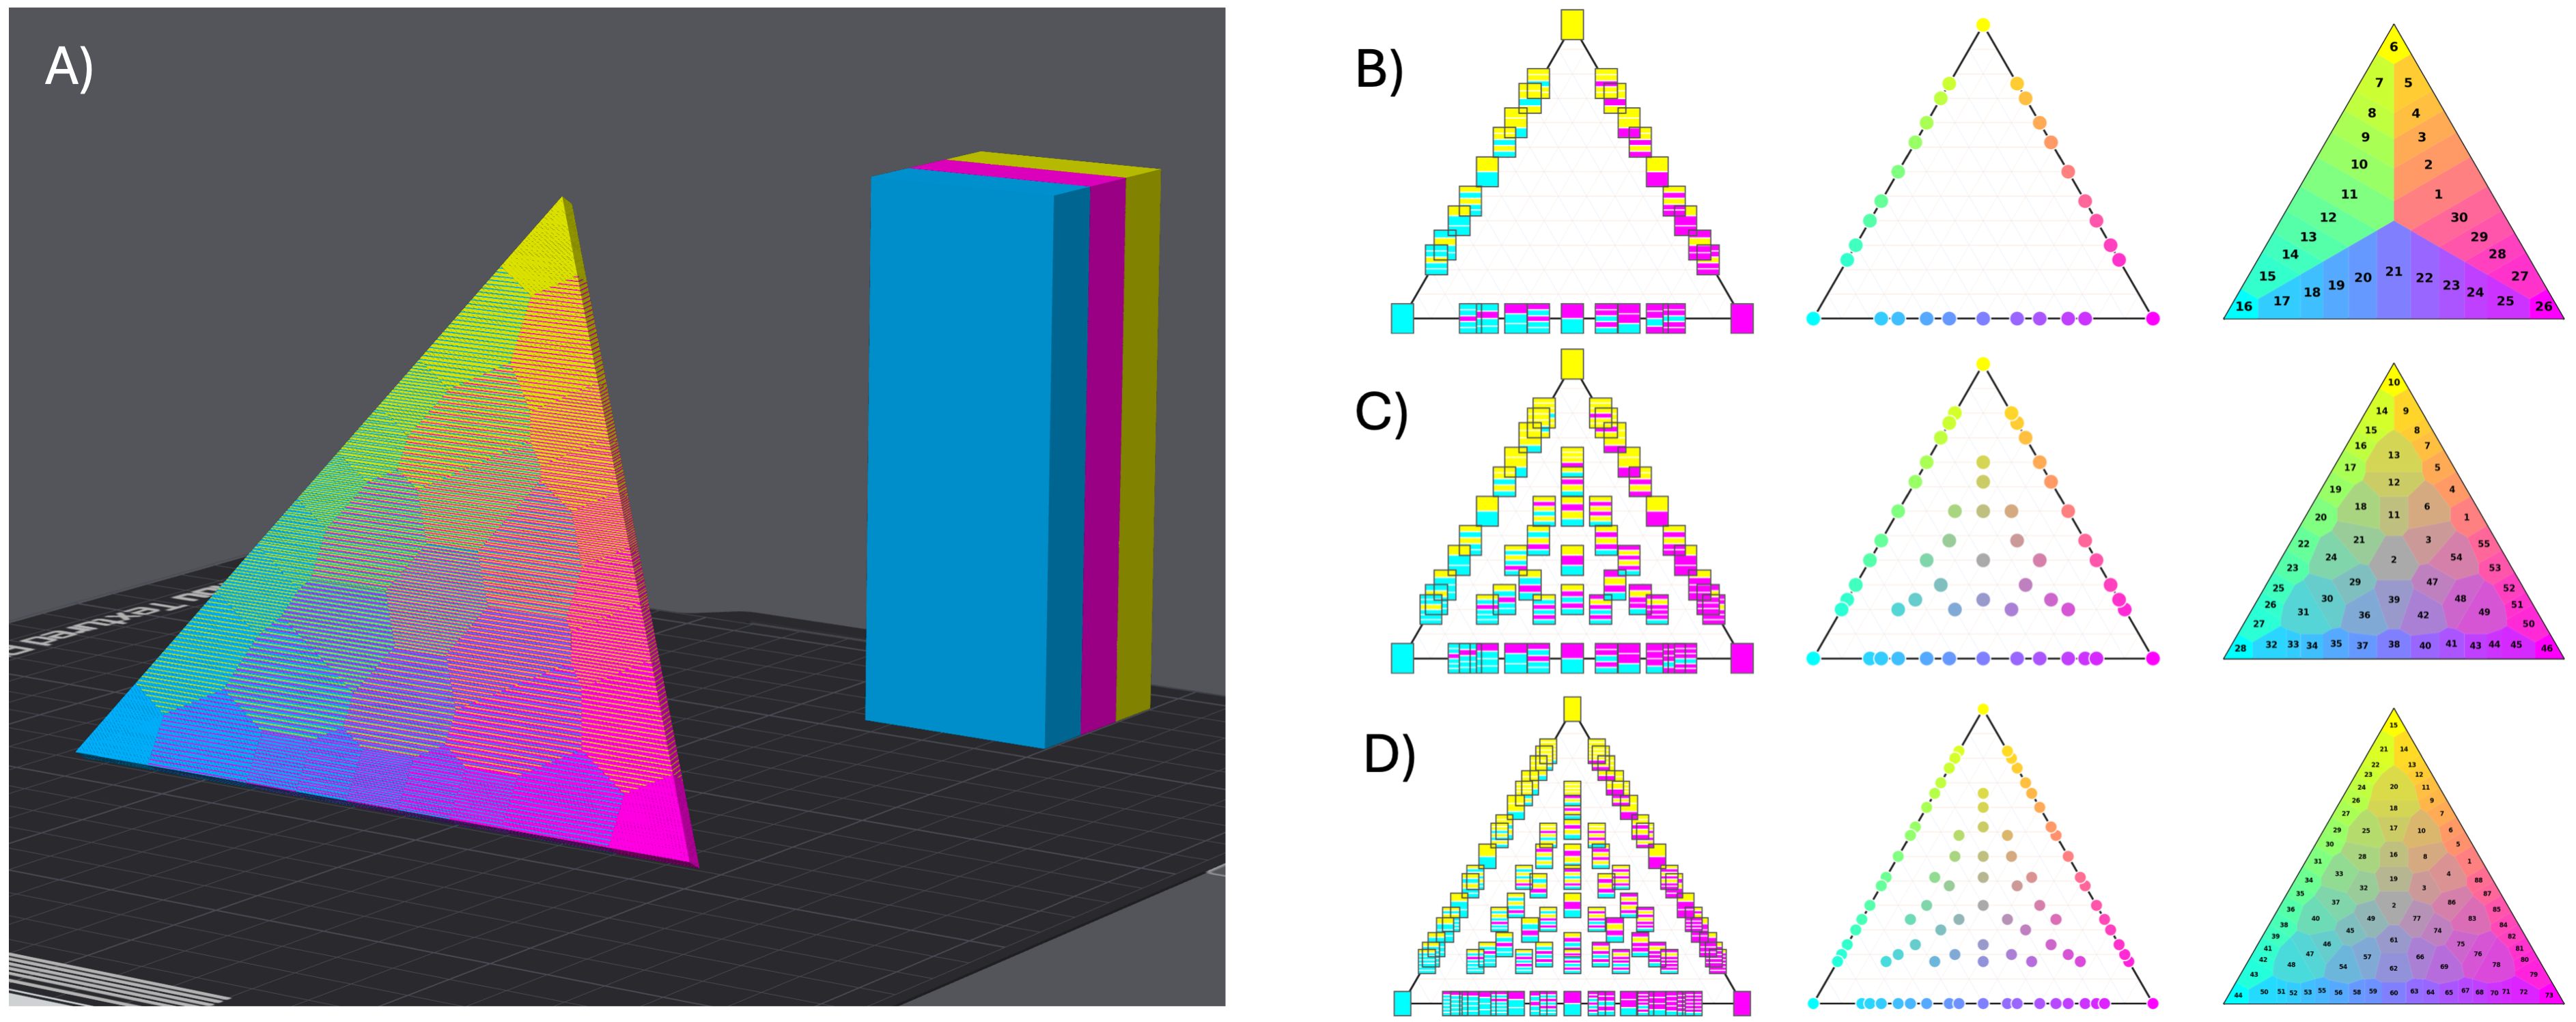
\includegraphics[width=0.95\linewidth]{fig02_cmy_weave_composition_voronoi.png}
    \caption{
    \textbf{CMY weave Voronoi gamuts under three palette constraints.} \textbf{A}, a printed triangular CMY gamut and a three-filament reference object. \textbf{B--D}, successively denser palette constraints: \textbf{B}, maximum token height 6, written-token run limit 2, and at most 2 distinct colors; \textbf{C}, maximum token height 6, run limit 3, and at most 3 distinct colors; \textbf{D}, maximum token height 7, run limit 6, and at most 3 distinct colors. Within each of \textbf{B--D}, the three columns show layered tile stacks, solid-color sites in ternary CMY space, and numbered Voronoi regions indicating nearest-recipe partitions.
}
    \label{fig:cmy-voronoi}
\end{figure*}

The primary design tradeoff is between palette density and visible striation.
Striation increases with layer height and depends strongly on surface orientation, as shown by gamuts printed at 10$^\circ$, 45$^\circ$, and 90$^\circ$ (Fig.~\ref{fig:surface-angle}; Fig.~S7).
Reducing layer height visibly improved integration: patterns that showed stronger striping at 0.12~mm appeared smoother at 0.08~mm, and 0.16~mm Benchy prints showed the strongest layer visibility (Fig.~S8).
Rotating models so that broad surfaces are not perpendicular to the build plate also improves visual integration (Fig.~\ref{fig:surface-angle}B).
Striation varies across gamut space, with repeated same-color layers and high-contrast neighboring filaments revealing the woven structure most strongly.
\begin{figure*}[!t]
    \centering
    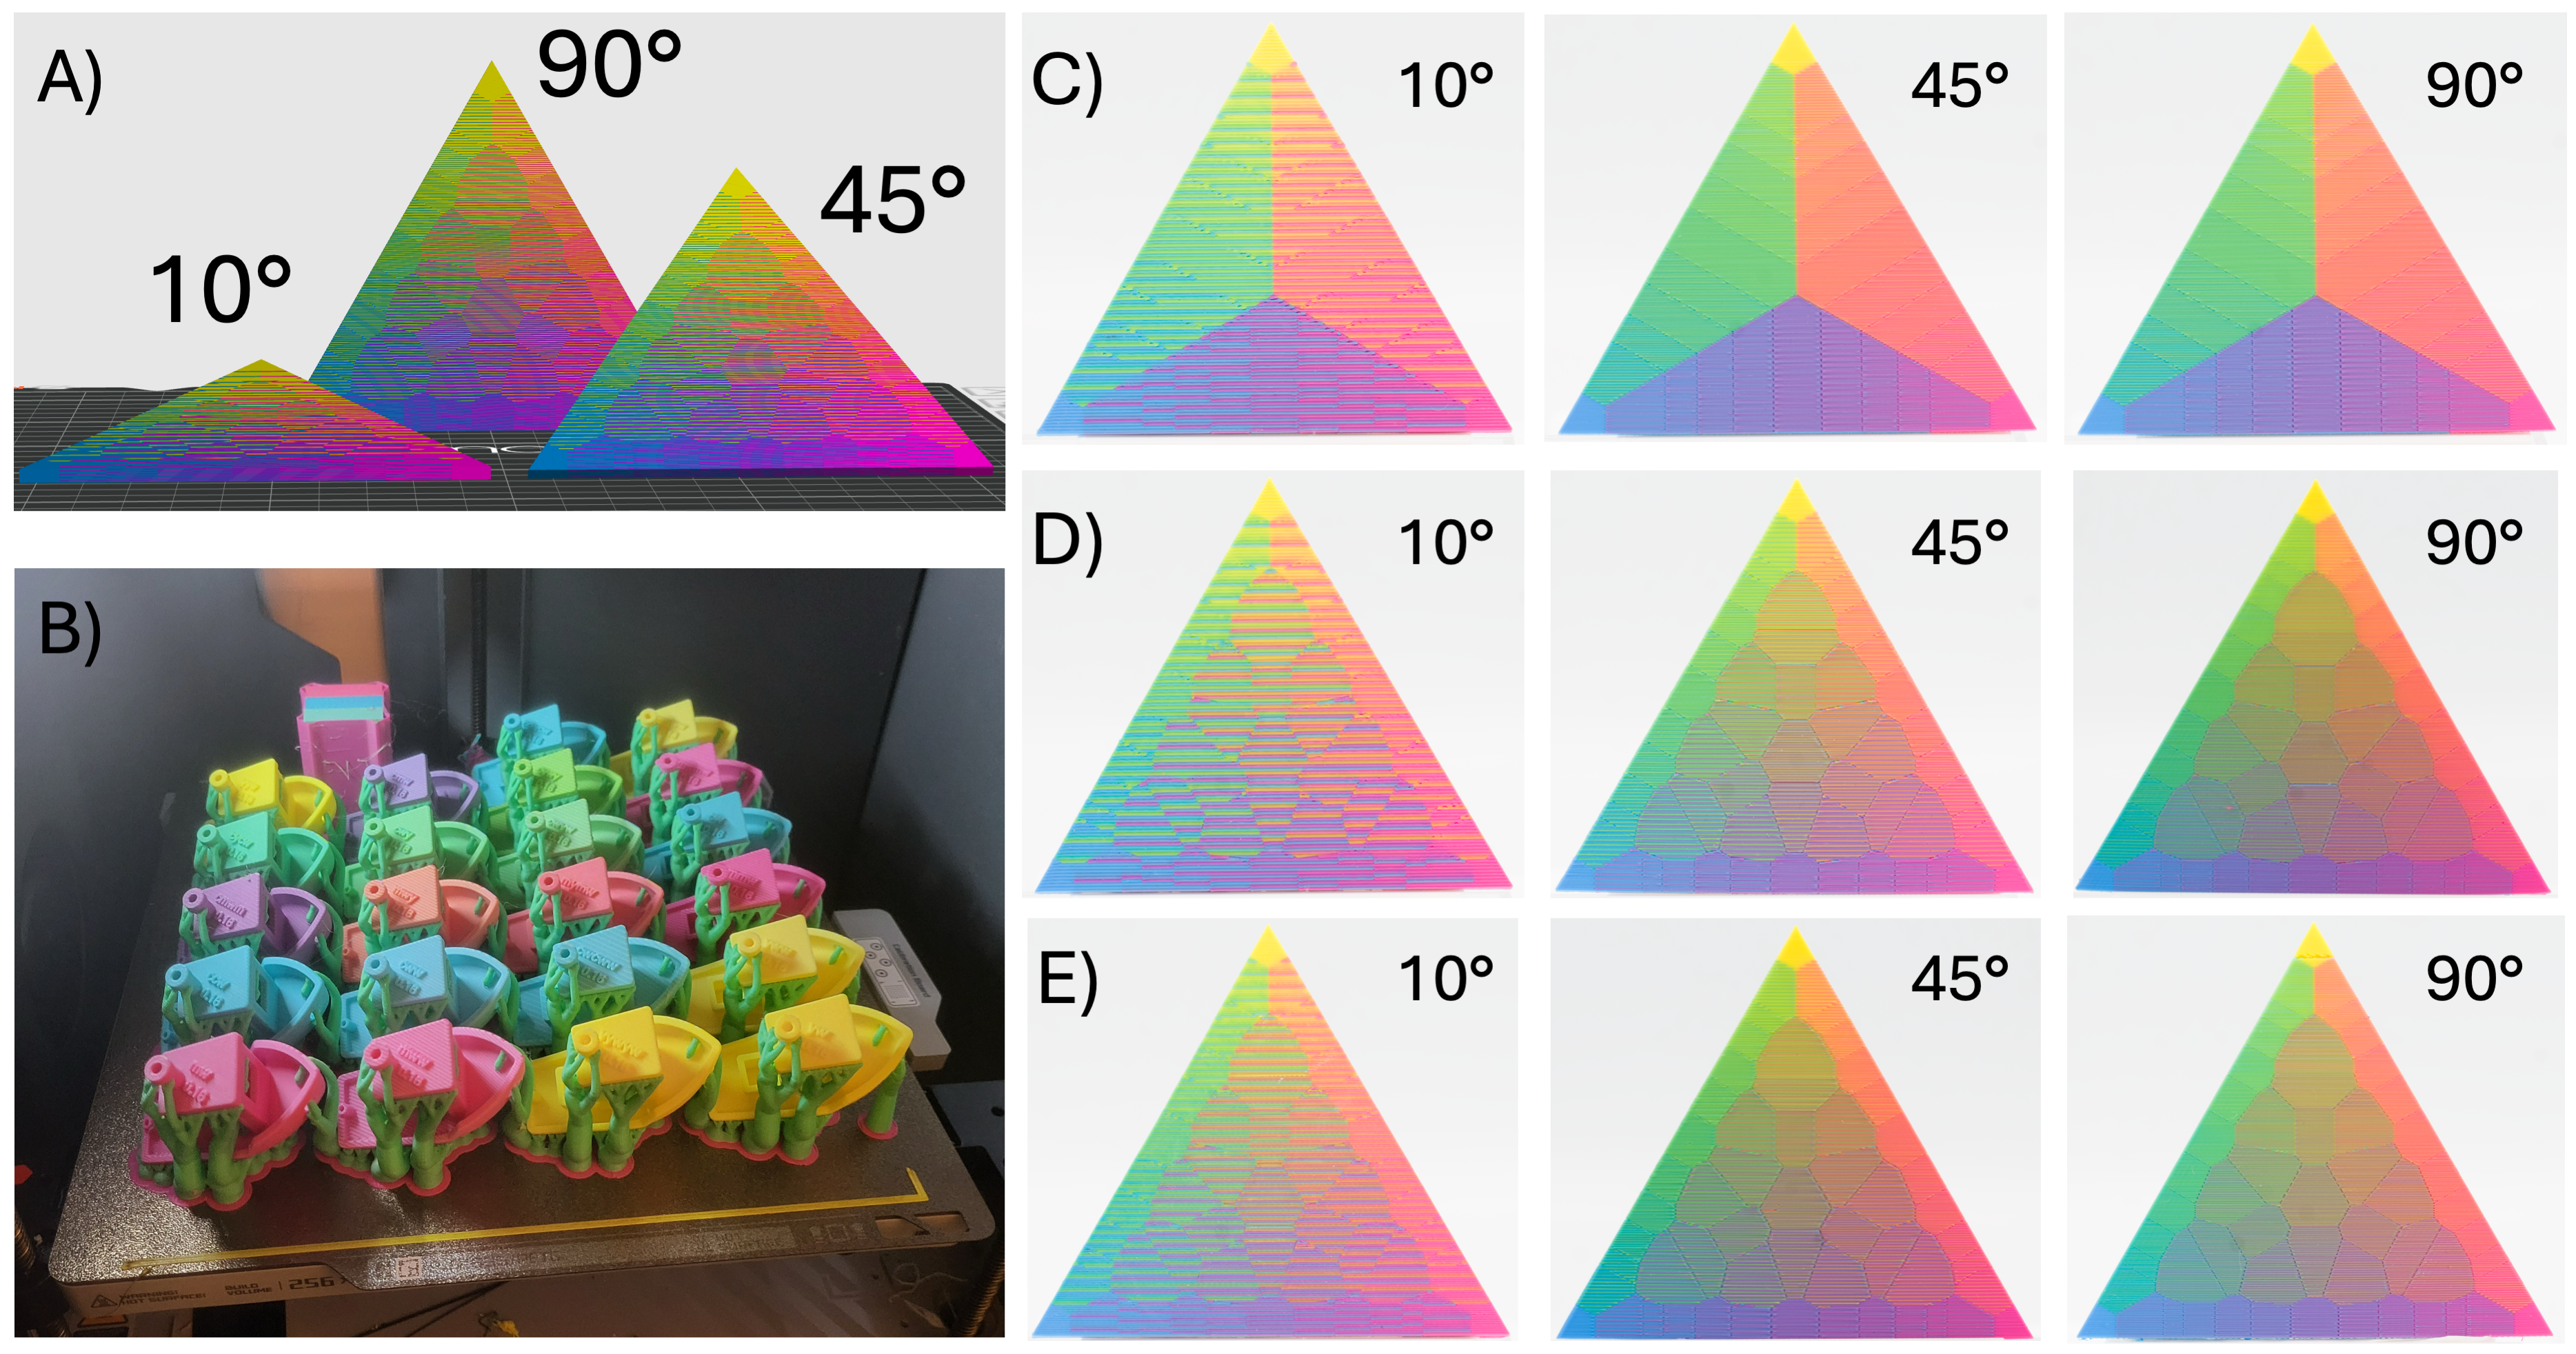
\includegraphics[width=0.95\linewidth]{fig03_orientation_striation_effects.png}
    \caption{
    \textbf{Surface orientation and weave complexity control visible striation.}
    \textbf{A}.
The same woven triangular gamut arranged at different build orientations illustrates how low-angle surfaces expose the Z-layer sequence, whereas steeper orientations visually integrate the woven layers more effectively.
\textbf{B}. A build plate of 3DBenchy orientation tests used to evaluate how non-planar surfaces expose woven layers.
\textbf{C--E}. Controlled triangular gamut samples printed at 0.12 mm layer height and tilted by 10$^\circ$, 45$^\circ$, and 90$^\circ$.
Rows compare increasing palette-complexity constraints: \textbf{C}, $(6,2,2)$; \textbf{D}, $(6,3,3)$; and \textbf{E}, $(7,6,3)$, where the tuple denotes maximum stack height, maximum repeated-color run length in the written token, and maximum number of distinct colors.
Longer or more complex weave patterns increase accessible recipe density but can make layer structure more visible, especially on shallow surfaces.
}
    \label{fig:surface-angle}
\end{figure*}

\subsection{Application Models and Visible Striation}

To evaluate LayerLoom on practical printed geometries beyond flat gamut samples, we tested 107 weave patterns using CMYKW colors at a 0.16~mm layer height;
the endpoint filaments are listed in Table~S5, and the Benchy gallery is shown in Fig.~S8.
3DBenchy was used as a familiar benchmark geometry for assessing visible striation on non-planar surfaces \citep{creative_tools_3dbenchy_2015}.
Two-color weaves at the smallest tested layer height produced the smoothest results.
The Benchy prints reproduced the orientation-dependent striation trends observed in the gamut samples: sidewalls blended more smoothly, whereas top and bottom surfaces exposed the layer sequence more strongly.
Lower-contrast, lower-layer-height models showed the least striation.


Scientific visualization is a natural use case because many models require more color-coded categories than available filament slots.
We applied LayerLoom to protein-structure visualizations generated from RMSX and Flipbook molecular-dynamics snapshots \citep{beruldsen2026rmsx}.
The snapshots were exported from ChimeraX as GLB files \citep{meng2023chimerax}, imported into LayerLoom, automatically mapped to woven recipes from their GLB color information, and sliced in OrcaSlicer at a 0.12~mm layer height.
The final prints preserved the main regions of higher and lower molecular motion, with the strongest striation again appearing on regions perpendicular to the build plate (Fig.~\ref{fig:applications}A--B).
LayerLoom also supports color-coded 3D graphics and anatomical models, where discrete regions may require more displayed colors than the number of loaded filaments, as shown in the foot skeleton example (Fig.~\ref{fig:applications}D--E).
These examples show how woven color can encode semantic categories without assigning each category to a separate physical material.
\begin{figure*}[!t]
    \centering
    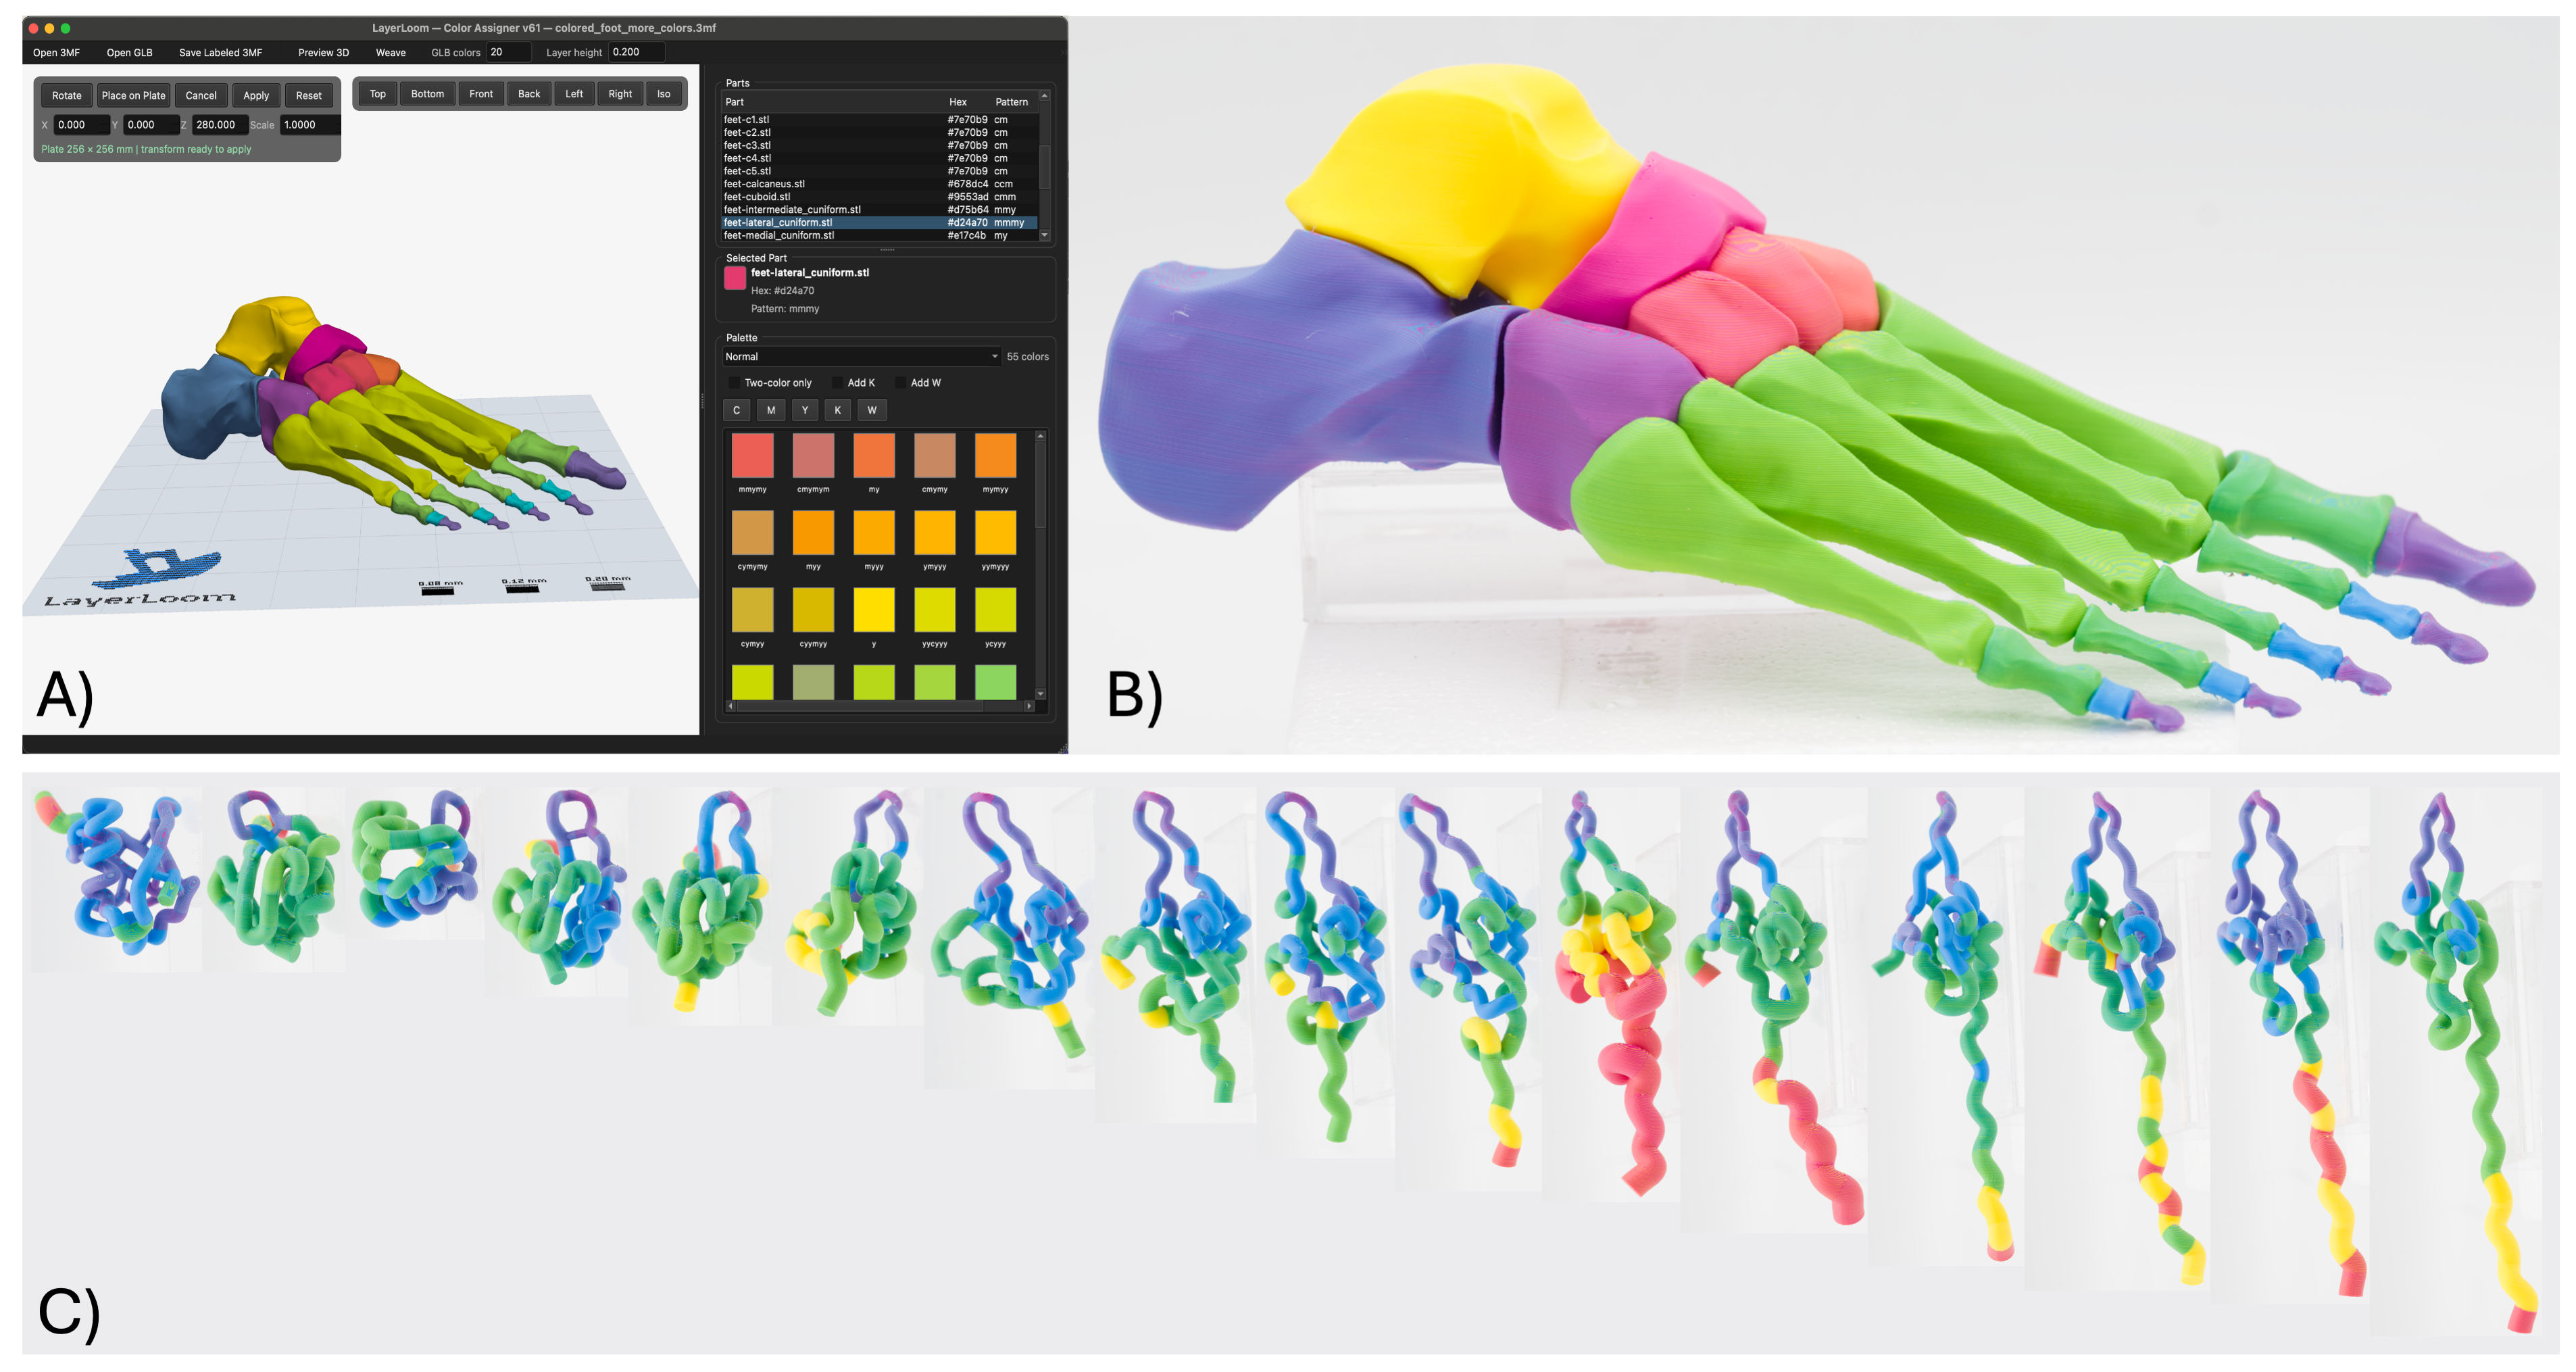
\includegraphics[width=0.95\linewidth]{fig04_applications_scientific_visualization.png}
    \caption{
    \textbf{LayerLoom applied to scientific and anatomical visualization.}
    \textbf{A}.
Printed protein-structure snapshots generated with RMSX/Flipbook from NAMD molecular-dynamics trajectories \protect\citep{beruldsen2026rmsx}.
\textbf{B}. Corresponding molecular visualization frames exported from ChimeraX \protect\citep{meng2023chimerax}.
\textbf{C}. 3DBenchy gallery illustrating woven recipes across many color combinations and surface orientations.
\textbf{D}. LayerLoom graphical interface for assigning woven color recipes to imported model components, shown with a color-coded human foot skeleton model.
\textbf{E}. Printed human foot skeleton model adapted from Printables \protect\citep{printables2024feet}.
Eleven displayed colors distinguish major hindfoot, midfoot, and forefoot structures despite using only three physical CMY filaments.
}
    \label{fig:applications}
\end{figure*}

\subsection{Benchmark Measurements Show Low Overhead When Woven Colors Reuse Existing Filaments}

This benchmark tests whether adding displayed woven colors has lower overhead when the new colors reuse filaments already required by the print.
We generated five 3-by-3 cube-array arrangements, with each cube having a 15~mm edge length and a 3~mm gap between neighboring cubes.
This produced a total model footprint of 51~$\times$~51~$\times$~15~mm.
Arrangement A1 is the baseline plate with direct filament assignments.
Arrangements A2 and A3 add woven-color cubes made from the same physical filaments already active in A1.
Arrangements A4 and A5 add a new physical filament color, so they isolate the cost of increasing the physical filament-channel count.

For each model arrangement (Fig.~\ref{fig:performance}; Table~S3), models were sliced using a 0.12~mm layer height.
Unless otherwise noted, slicer-default process settings were used, including 15\% infill; the Bambu Studio project metadata records two wall loops.
We compared the multi-nozzle Snapmaker U1, the multi-tool Prusa XL, and the filament-swapping Bambu Lab X1C.
Snapmaker U1 and Bambu Lab X1C values were measured from completed prints, including actual elapsed print time and total filament use recorded for each build.
Prusa XL values were included as PrusaSlicer 2.9.4 estimates to compare the same benchmark arrangements on a second multi-tool workflow.
Since PrusaSlicer did not include a default 0.12~mm profile for the Prusa XL, we modified the 0.10~mm DETAIL profile to use a 0.12~mm layer height.
These measurements and estimates test a specific practical consequence of geometry-encoded layer scheduling: slicers plan toolpaths according to the physical filament assignments present on each layer.
Across the tested workflows, the smallest overhead was observed when woven components reused physical filaments that were already required on the same layers of the build (Fig.~\ref{fig:performance}A--B).
This comparison is represented by A1 versus A2 and A1 versus A3, where additional woven colors are introduced without requiring an additional physical filament channel.

The effect was clearest for the multi-nozzle and multi-tool workflows: the Prusa XL estimates were essentially unchanged from A1 to A3, and the measured Snapmaker U1 changes were small. The filament-swapping Bambu X1C showed larger time and material differences, consistent with the higher cost of material switching on single-nozzle systems, but the largest increase occurred when an additional physical filament was introduced rather than when additional woven recipes reused already loaded base filaments. Together, these benchmarks separate displayed color count from physical filament count: when woven colors reuse filaments already active on the relevant layers, additional displayed colors can be introduced with comparatively small overhead.



\begin{figure*}[!t]
    \centering
    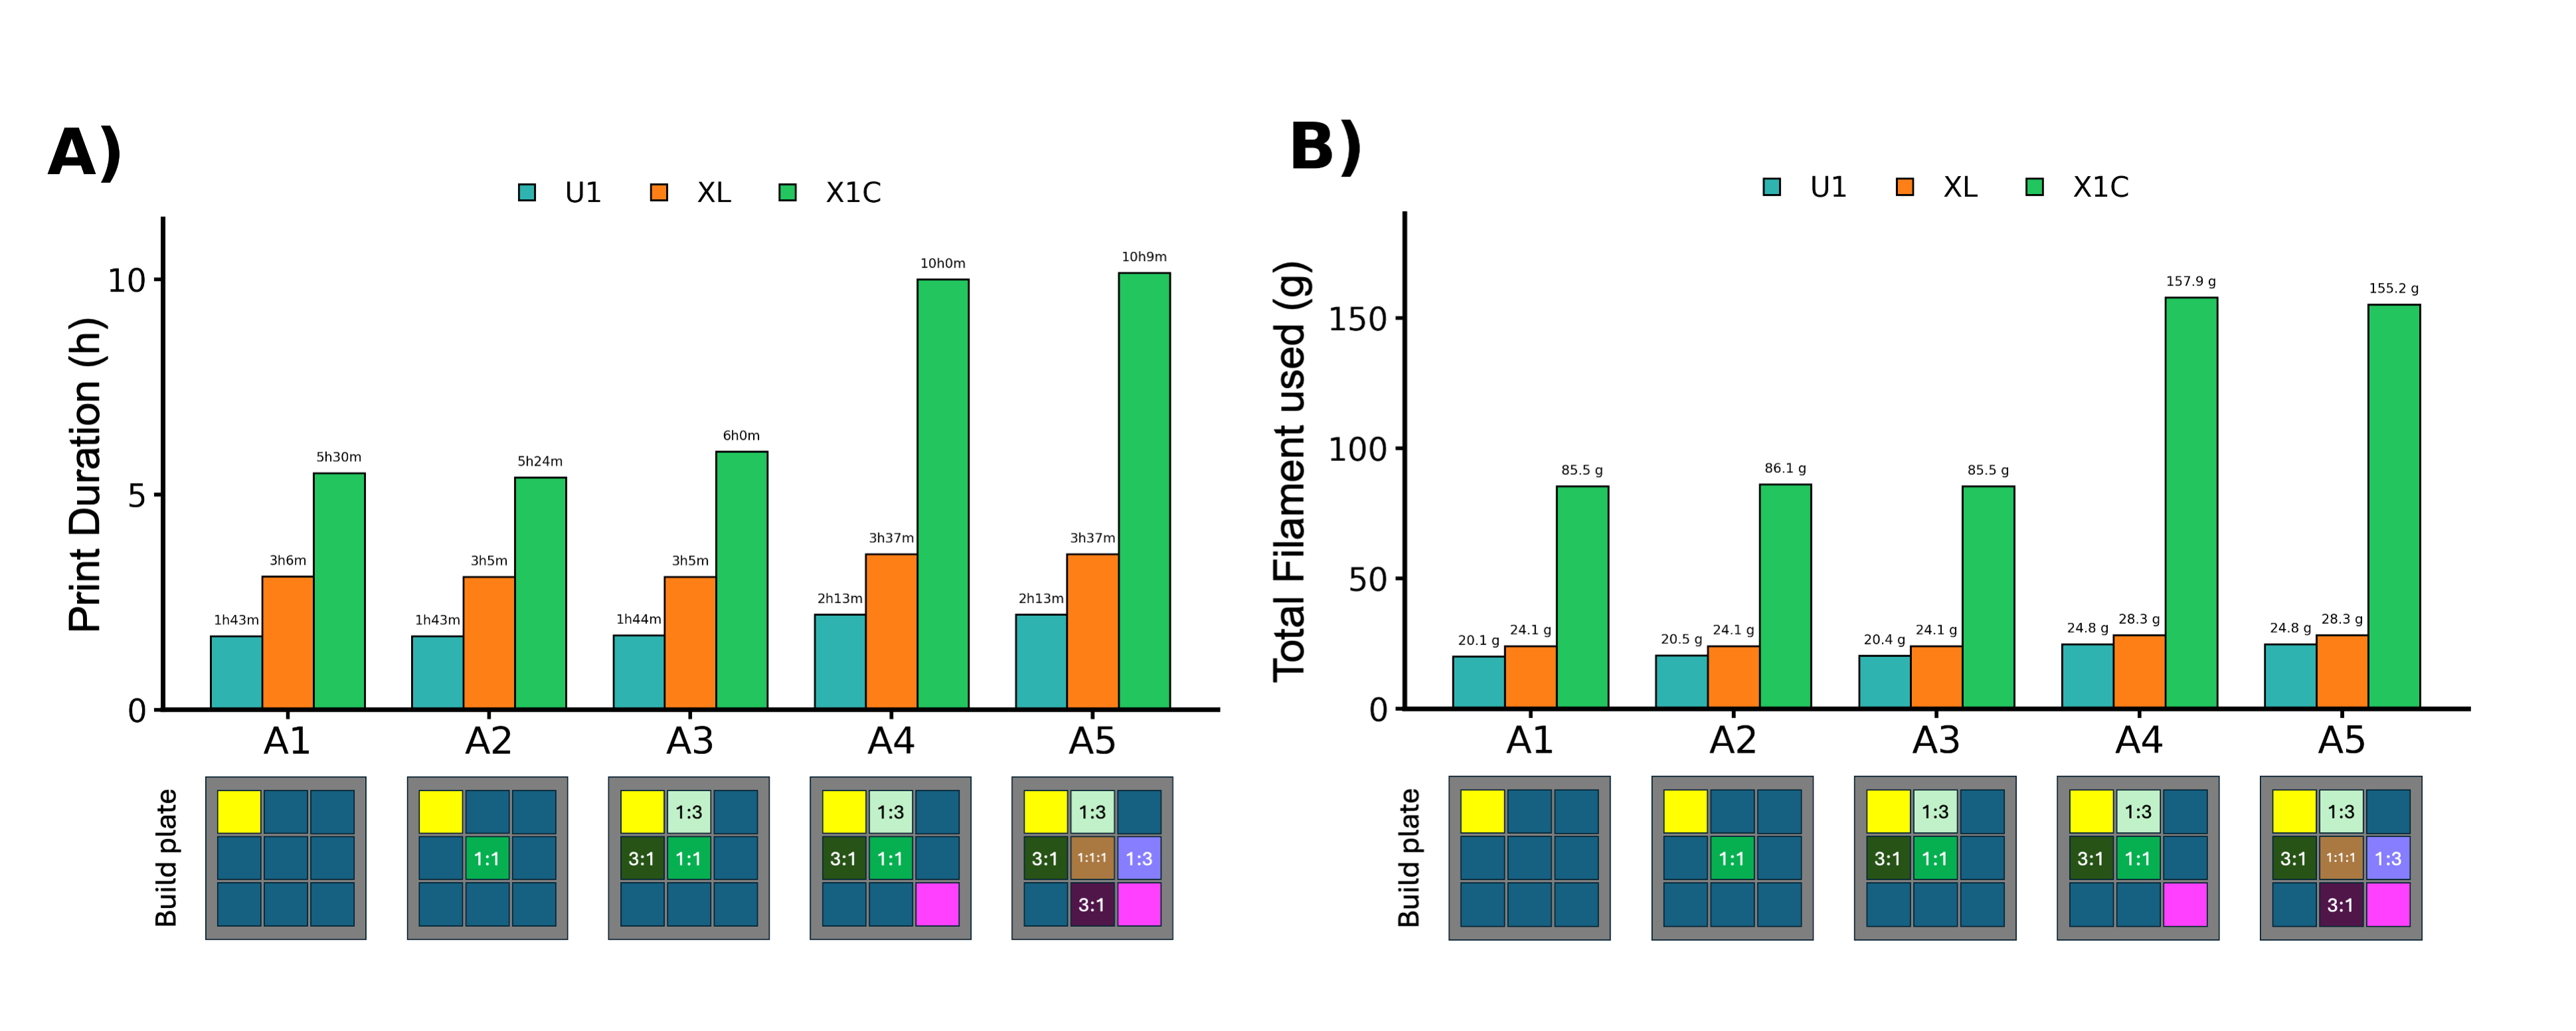
\includegraphics[width=0.95\textwidth]{fig05_time_filament_benchmark.png}
    \caption{
    \textbf{Print time and material use for nine-cube multi-material benchmarks.}
    Five 3-by-3 cube-array arrangements were compared on the Snapmaker U1, Prusa XL, and Bambu Lab X1C.
Cubes are 15~mm per edge and were sliced at 0.12~mm layer height with two exterior walls. \textbf{A}, print time in hours. \textbf{B}, total filament used in grams.
A1 is the direct-color baseline, A2--A3 add woven colors while reusing already loaded filaments, and A4--A5 introduce another physical filament color.
In these benchmarks, woven colors impose the least overhead when they reuse filaments already required by the print.
Snapmaker U1 and Bambu Lab X1C values are measured from completed prints; Prusa XL values are slicer estimates.
}
    \label{fig:performance}
\end{figure*}

\subsection{Expanded Secondary and Neutral Endpoints}

The CMY tests demonstrate the basic layer-weaving principle, but any loaded filament can serve as an endpoint in the same token grammar. We tested this broader palette by replacing one CMY endpoint at a time with white, light gray, dark neutral gray, black, orange, violet, or green (Fig.~\ref{fig:ovg-neutral-mosaic}; Figs.~S1--S3; Table~S5). These secondary and neutral/value endpoints extend the available color space and provide the printed source data for the calibrated color-coverage analysis. Table~\ref{tab:palette-family-counts} summarizes how the theoretical recipe space grows as additional endpoints are made available.

\begin{figure*}[!t]
    \centering
    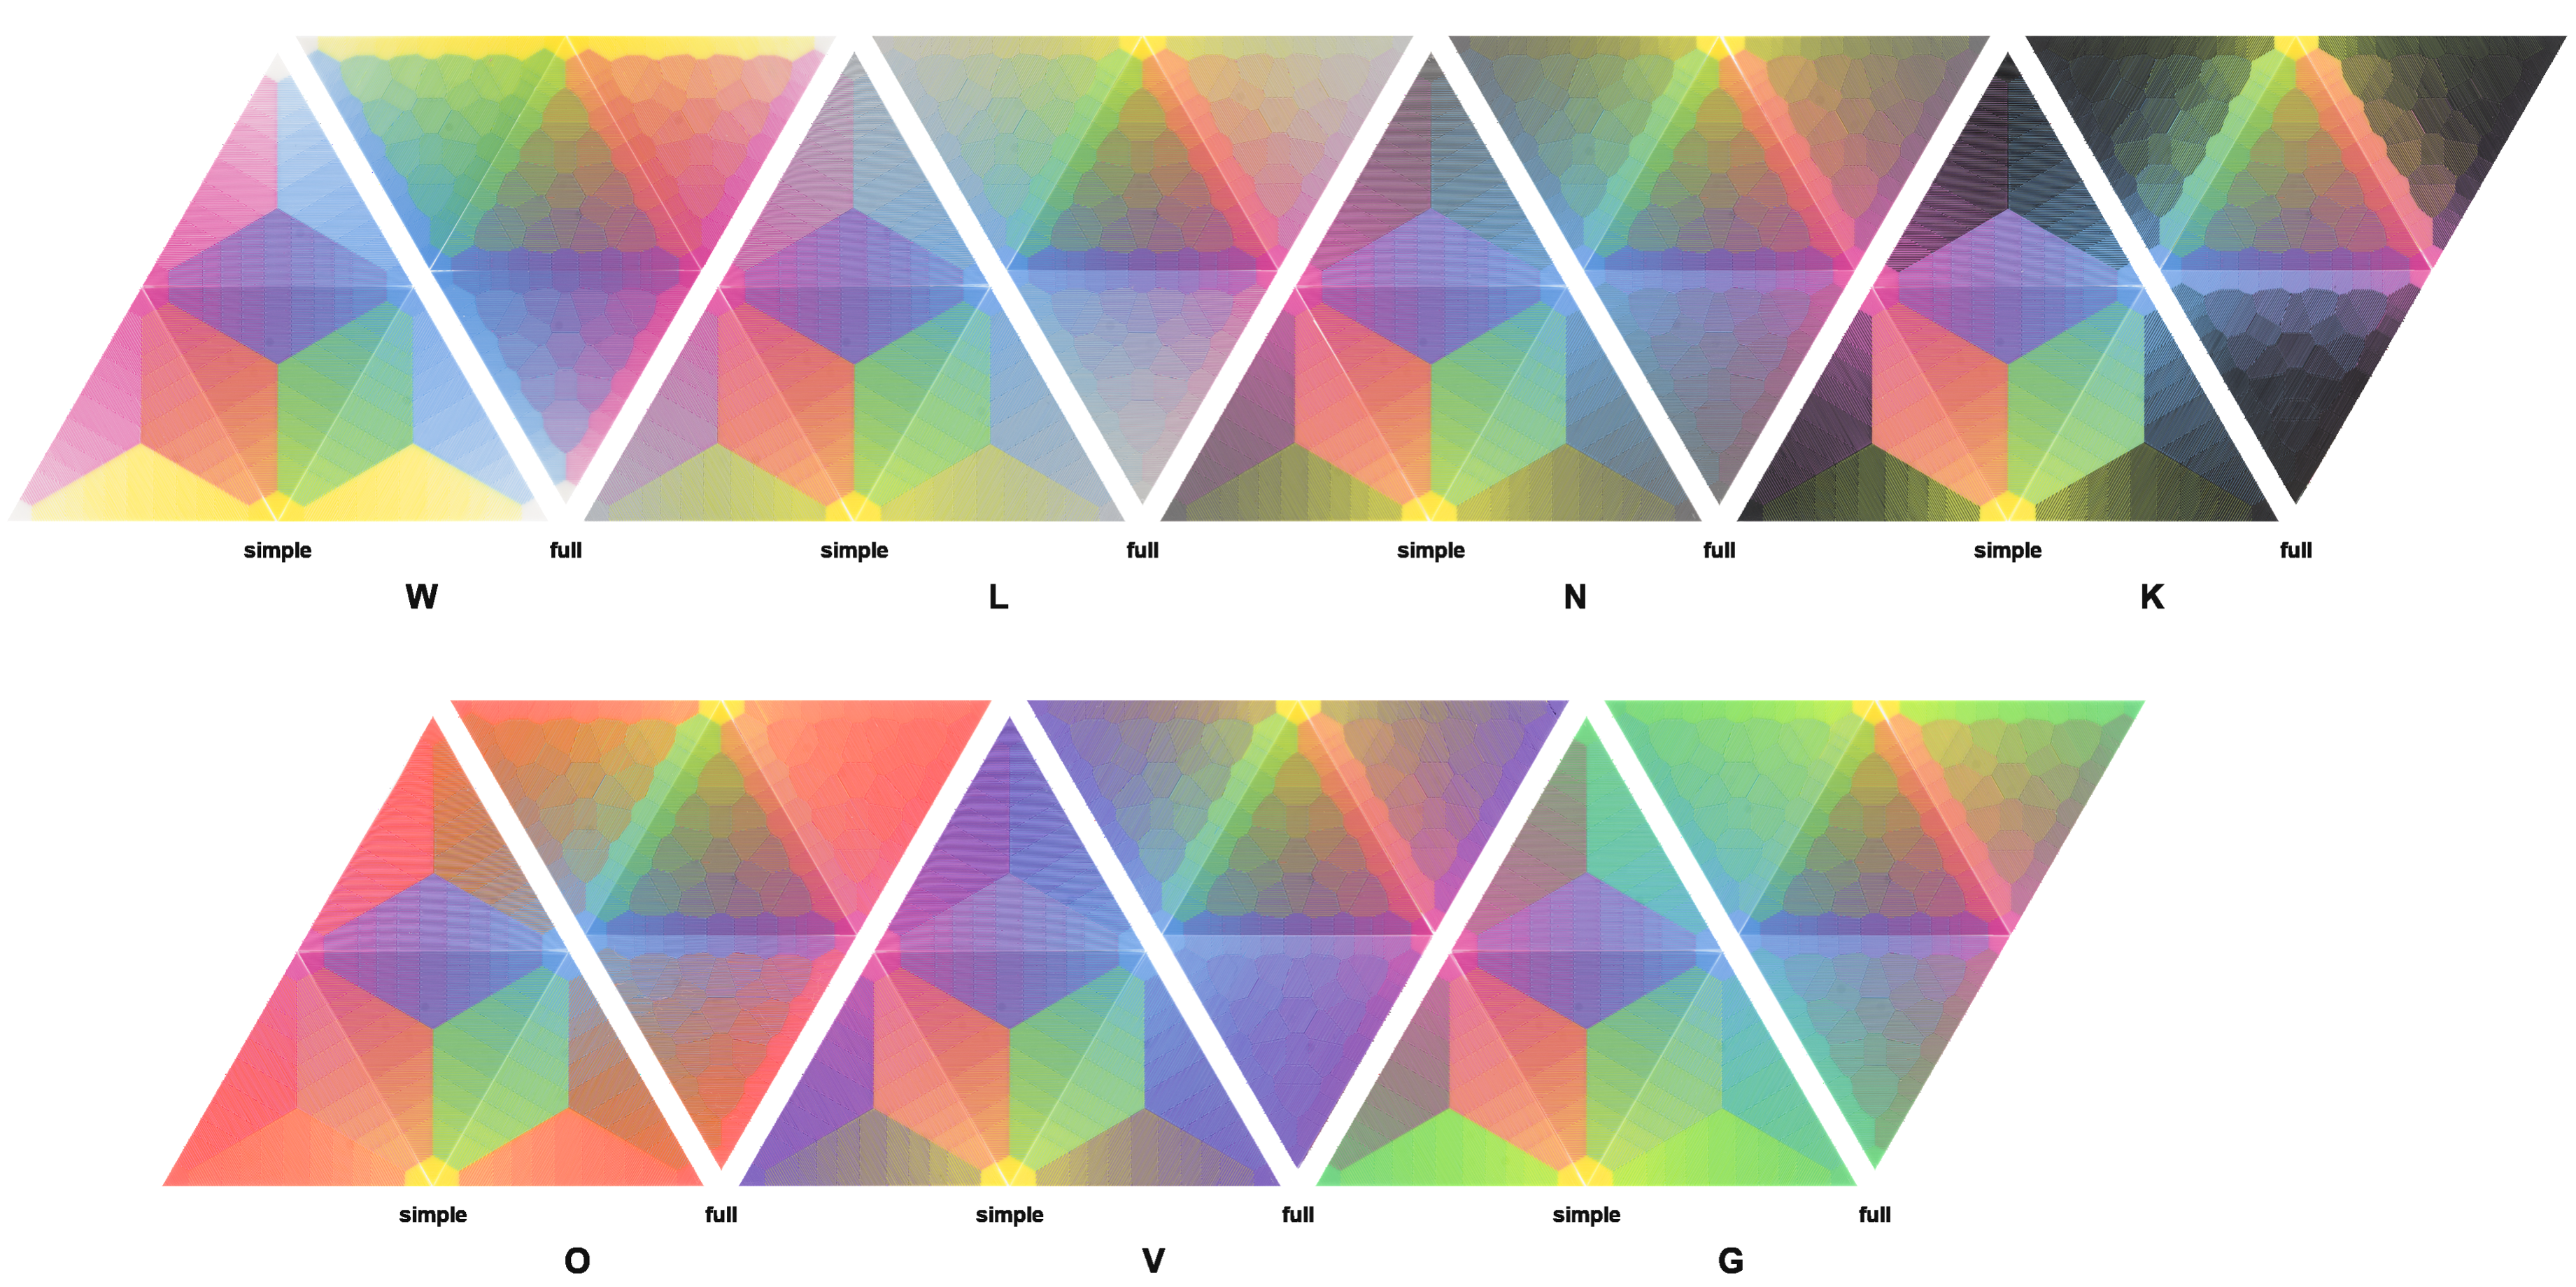
\includegraphics[width=0.95\linewidth]{fig06_cmykw_ovg_neutral_mosaic.png}
    \caption{
    \textbf{Expanded woven-color design spaces using neutral and secondary endpoints.}
    Each added filament is shown under the two-color and full printed-triangle weave rule sets. Triangular gamut objects retain two CMY endpoints and replace the third endpoint with the added filament: \textbf{W} white, \textbf{L} light gray, \textbf{N} dark neutral gray, \textbf{K} black, \textbf{O} orange, \textbf{V} violet, and \textbf{G} green. The full weave rule set adds denser interior recipes, showing how neutral/value and secondary endpoints expand the LayerLoom design space beyond CMY-only weaving.
}
    \label{fig:ovg-neutral-mosaic}
\end{figure*}

\subsection{Calibrated Image-Based Color Quantification of Printed Gamuts}

Printed gamut samples were quantified from calibrated photographs using a region-aware Python workflow (Figs.~\ref{fig:gamut-photo-analysis} and~\ref{fig:gamut-error-uniformity}; Supplementary Methods). Each photograph was color-corrected using a ColorChecker-based camera profile, registered to the expected LayerLoom region layout, and sampled from eroded interior masks to avoid seams, borders, shadows, layer-edge artifacts, and registration-sensitive boundaries. Median region colors were converted to CIE \(L^*a^*b^*\) and compared using CIEDE2000 distances \citep{iec_61966_2_1_1999,cie_11664_4_2019,cie_11664_6_2022,luo2001ciede2000,sharma2005ciede2000}. For each measured gamut set, chromatic coverage was summarized by the convex-hull area of the measured \(a^*b^*\) points, and color density was summarized by the median nearest-neighbor distance among measured points. Distinguishable color counts were computed by connecting regions with pairwise \(\Delta E_{00}\) below a threshold and counting the resulting graph components. For expanded endpoint analyses, the region counts represent printed observations pooled across three-endpoint substitution gamuts, not unique theoretical recipes from the full combined palette. Detailed camera settings, RAW processing, mask generation, pixel trimming, and repeatability checks are provided in the Supplementary Methods.
Using this calibrated image-based workflow, the two-color CMY gamut contained 30 measured regions and produced 30 distinguishable printed clusters at the strict threshold of \(\Delta E_{00}<2\), with a measured \(a^*b^*\) hull area of 6,226.
The full CMY gamut contained 55 measured regions and produced 51 distinguishable clusters at \(\Delta E_{00}<2\), with a hull area of 6,646.
Adding OVG endpoints under the full weave rule set increased the measured set to 495 regions, 152 distinguishable clusters, and a hull area of 8,146.
Adding neutral/value endpoints under the full weave rule set increased the measured set to 660 regions, 298 distinguishable clusters, and a hull area of 7,042.
The combined expanded endpoint set under the full weave rule set contained 1,210 measured regions, produced 393 distinguishable clusters at \(\Delta E_{00}<2\), and reached a hull area of 8,752 (Fig.~\ref{fig:gamut-photo-analysis}; Table~S2; Figs.~S4--S6).
The median nearest-neighbor distance decreased from 6.48 \(a^*b^*\) units for full CMY to 1.57 for the combined expanded endpoint set, indicating increased measured color density as well as expanded coverage.
Repeat photographs supported the stability of the calibrated image workflow (Table~S4).
The duplicate full-rule-set \texttt{ywm} pair was mostly below \(\Delta E_{00}=1\), with the largest region difference approximately 1.20, and the duplicate two-color CMY pair showed similarly low differences.
These repeatability checks indicate that the registered, calibrated photographic workflow was stable for relative comparisons among printed gamut samples.
Figure~\ref{fig:gamut-error-uniformity} separates nominal palette error from local print uniformity in the simple and full CMY gamuts.
The \(\Delta E_{00}\) maps and expected-to-measured \(a^*b^*\) shift plots show that measured colors do not follow a calibrated linear optical mixture model.
In particular, the cyan endpoint appears darker and bluer than the nominal reference, and yellow-rich mixtures shift substantially when even small amounts of magenta or cyan are introduced.
Thus, increased layer fraction does not move printed colors linearly toward the expected vertex colors.
These deviations are useful diagnostically: they show that LayerLoom can generate many distinguishable printed colors, while accurate target matching will require empirical or calibrated palette selection.
Image analysis and plotting were performed in Python using NumPy, pandas, and Matplotlib \citep{harris2020numpy,mckinney2010pandas,hunter2007matplotlib}.
Because all samples were processed through the same calibrated imaging and analysis workflow, these measurements provide a calibrated, repeatable basis for comparing relative gamut coverage, distinguishable color count, local uniformity, and measured color density across printed designs.
\begin{figure*}[!t]
    \centering
    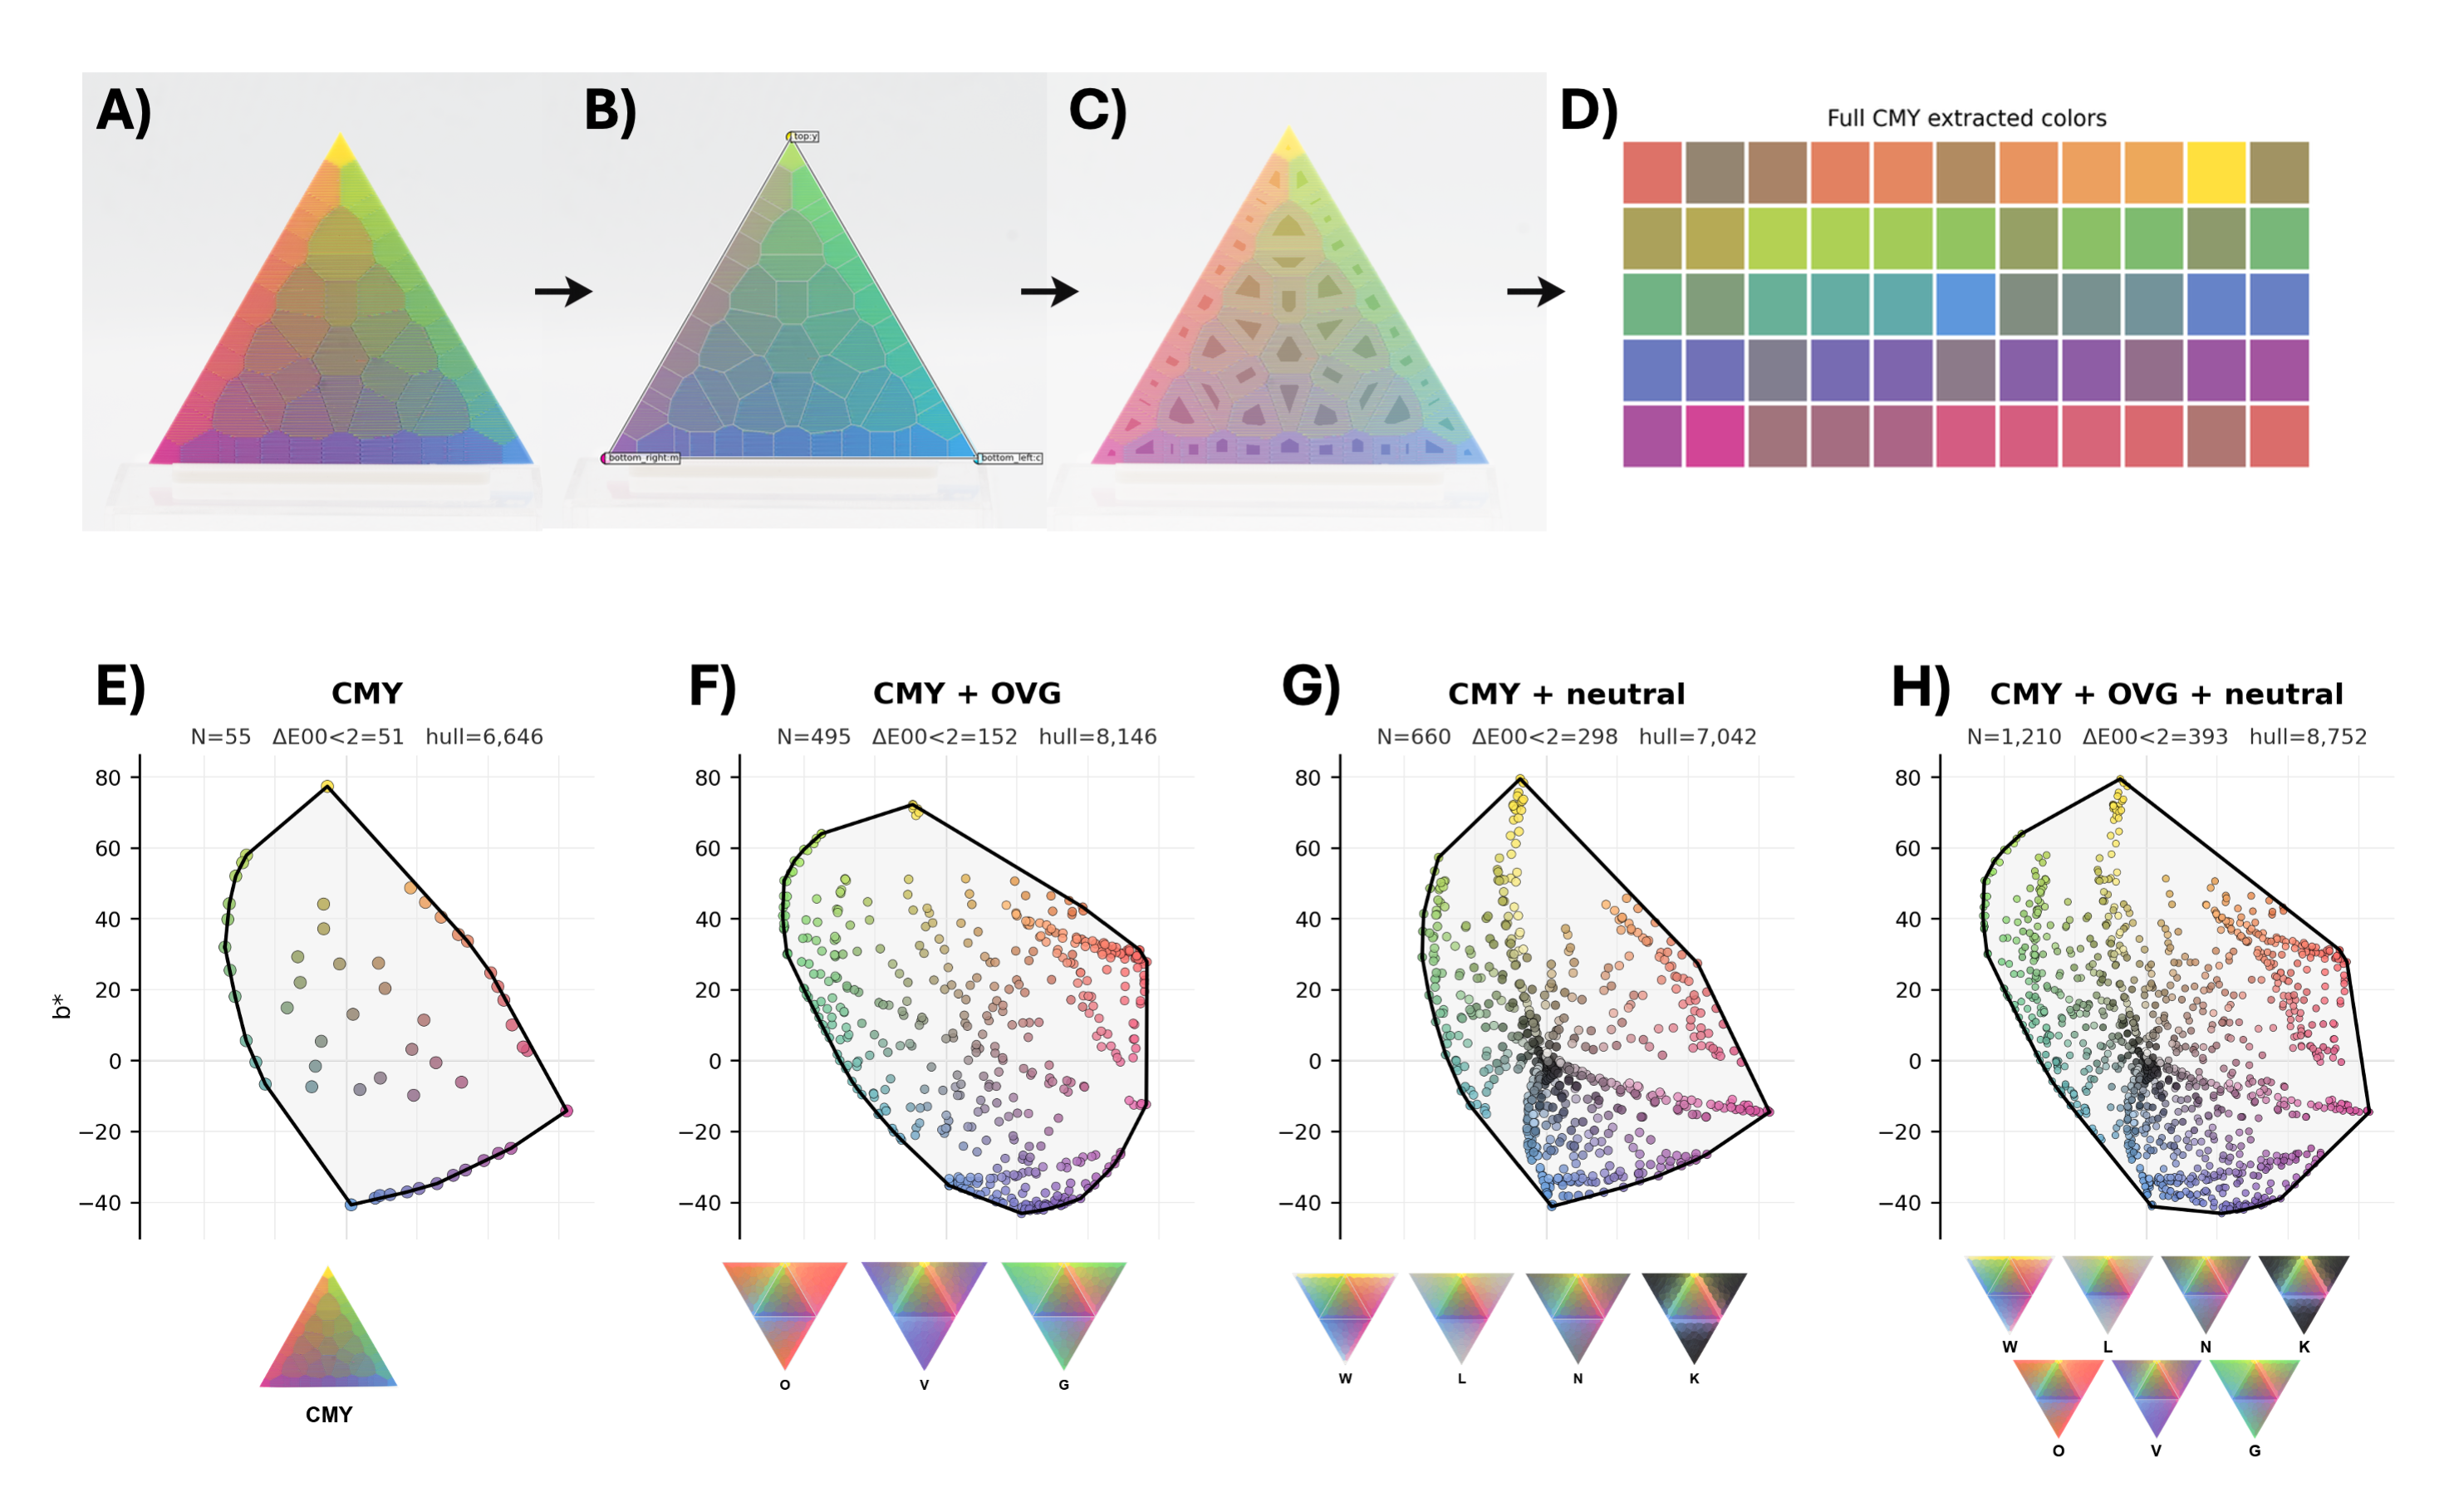
\includegraphics[width=0.98\linewidth]{fig07_image_color_quantification_workflow.png}
    \caption{
    \textbf{Calibrated image-based analysis of printed LayerLoom color coverage.}
    \textbf{A--D}.
Region-based image-analysis workflow for the full CMY gamut sample. \textbf{A}. Calibrated photograph. \textbf{B}. Expected LayerLoom regions registered to the photograph.
\textbf{C}. Interior sampling masks used to exclude seams, borders, shadows, and edge-registration artifacts. \textbf{D}.
Median extracted color for each registered region.
    \textbf{E--H}. Measured CIE \(a^*b^*\) coverage for printed gamut sets generated with the full printed-triangle weave rule set \((H \leq 6,\ \mathrm{run} \leq 5,\ \leq 3\ \mathrm{endpoint\ colors})\).
Points indicate median printed-region colors, and black outlines indicate measured convex hulls.
Per-panel annotations report measured regions, distinguishable clusters at \(\Delta E_{00}<2\), and measured hull area. \textbf{E}. CMY baseline. \textbf{F}.
CMY plus orange, violet, and green. \textbf{G}. CMY plus white, light gray, dark neutral gray, and black. \textbf{H}.
Combined CMY, OVG, and neutral/value endpoints. Source strips below each plot show the printed samples included in each measurement set.}

    \label{fig:gamut-photo-analysis}
\end{figure*}

\begin{figure*}[!t]
    \centering
    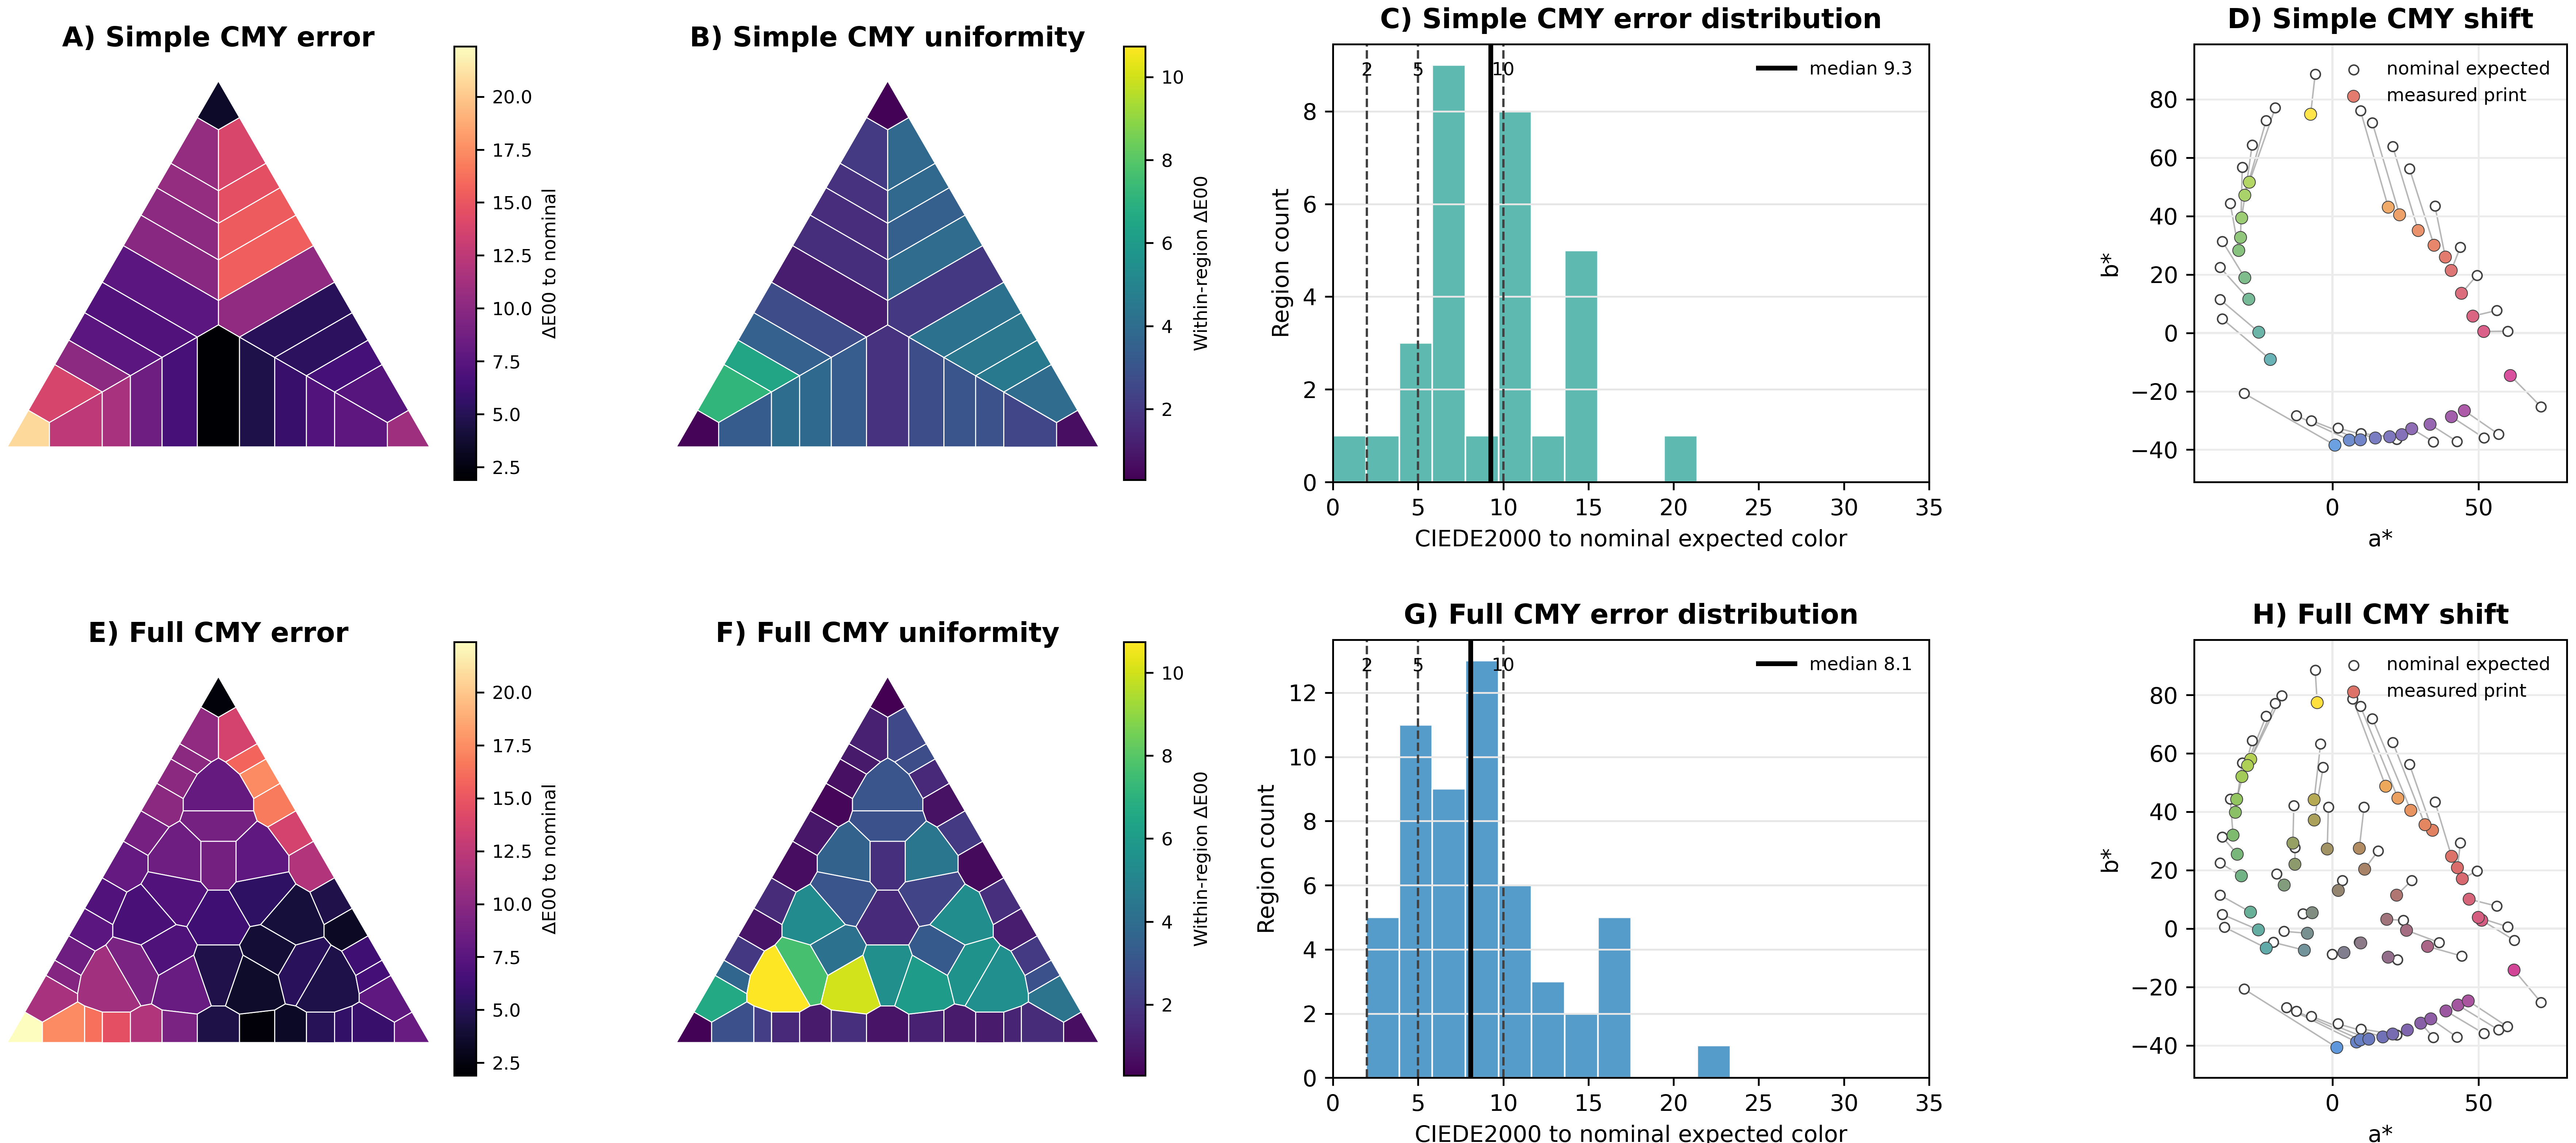
\includegraphics[width=0.98\linewidth]{fig08_cmy_color_error_uniformity.png}
    \caption{
    \textbf{Diagnostic color error, local uniformity, and expected-to-measured shifts for CMY gamuts.} \textbf{A--D}.
Two-color CMY gamut generated with the restricted printed-triangle rule set \((H \leq 6,\ \mathrm{run} \leq 2,\ \leq 2\ \mathrm{endpoint\ colors})\).
\textbf{A}. Spatial map of CIEDE2000 color difference, \(\Delta E_{00}\), between each measured printed region and its nominal expected CMY color.
\textbf{B}. Within-region color variation, computed as the median \(\Delta E_{00}\) distance between sampled pixels and the median color of that region.
\textbf{C}. Distribution of region-level \(\Delta E_{00}\) errors. Dashed reference lines mark \(\Delta E_{00}=2\), \(5\), and \(10\), and the solid line marks the median error.
\textbf{D}. Expected-to-measured shifts in CIE \(a^*b^*\) space.
\textbf{E--H}. Full CMY gamut generated with the denser printed-triangle rule set \((H \leq 6,\ \mathrm{run} \leq 5,\ \leq 3\ \mathrm{endpoint\ colors})\).
\textbf{E}. Spatial \(\Delta E_{00}\) error map. \textbf{F}. Within-region color variation. \textbf{G}. Distribution of region-level \(\Delta E_{00}\) errors. \textbf{H}.
Expected-to-measured shifts in CIE \(a^*b^*\) space.
}
    \label{fig:gamut-error-uniformity}
\end{figure*}


\section{Discussion}

LayerLoom shows that color expansion in multi-material FFF can be achieved by encoding layer structure directly into printable geometry. Its central contribution is a portable 3MF representation in which the model carries both the object shape and the layer sequence needed to fabricate each woven color. In the tested workflows, many woven recipes remained distinguishable after fabrication, showing that the expanded recipe space translated into practical printed colors.

These results distinguish recipe space, printed color separation, and target-color accuracy. LayerLoom expands the available layer-fraction recipes and produces many separated measured colors, while accurate target matching remains a separate color-management problem. The full CMY condition yielded 51 distinguishable clusters from 55 regions, and the combined expanded endpoint set yielded 393 clusters from 1,210 regions at \(\Delta E_{00}<2\). These counts show separability: many layer-fraction recipes produce different measured colors. The CMY diagnostic plots show where the nominal layer-fraction model diverges from measured printed colors, with the largest shifts near yellow-rich mixtures and around the cyan endpoint (Fig.~\ref{fig:gamut-error-uniformity}). This indicates that printed color does not follow a simple linear interpolation among nominal CMY vertices, as expected for real filaments whose pigment strength, opacity, scattering, and layer exposure differ among colors. Future versions of LayerLoom could use empirical filament-specific color maps to select weave recipes more accurately.

The dominant design tradeoff is between palette density and surface quality. Longer weave patterns provide more layer-fraction recipes, but they also make the material schedule more visible, particularly on surfaces that expose the Z-stack directly. Shorter patterns and lower layer heights reduced visible striation in the printed comparisons: 0.08~mm samples appeared cleaner than 0.12~mm samples, whereas the 0.16~mm Benchy prints showed stronger layer structure. The gamut samples and Benchy tests show that this trend is geometry-dependent. Vertical or steeply sloped sidewalls visually integrate alternating layers more effectively, whereas broad top or bottom surfaces expose the layer sequence.

LayerLoom's main advantage over slicer-native color-mixing workflows is that the material schedule is stored in the model rather than reconstructed by a specific slicer. Slicer-level systems can represent mixed colors as virtual materials during project setup, but the resulting schedule depends on that software's internal model and G-code generation. LayerLoom instead stores the repeated layer sequence directly in the 3MF as filament-specific geometry. Downstream slicers do not need to know what a woven color is; they need to preserve the generated Z positions at the weave height and map each output object to the intended physical filament. Under those compatibility conditions, the same woven model can transfer across ordinary multi-material slicers without specialized color-mixing hardware, custom feedstock, modified G-code, direct machine control, or slicer-specific mixed-color support.

The benchmark results reinforce the same point. Additional woven regions added the least overhead when they reused filaments already active on the relevant layers, while the largest increases in time and material use occurred when additional physical filament channels were introduced. This makes LayerLoom most useful for models where color is used to label information rather than to change material properties: scientific visualizations, anatomical models, educational objects, and color-coded prototypes.

Because LayerLoom varies the deposited color sequence while preserving the underlying polymer, woven and single-color coupons printed from the same PLA would be expected to have similar mechanical properties unless the alternating color interfaces weakened the part. Consistent with this expectation, we found no meaningful difference in ultimate tensile strength between woven and single-color coupons in either tested orientation (Supplementary Figs.~S9--S11 and Tables~S6--S7).

Overall, LayerLoom demonstrates that existing multi-material FFF printers can produce substantially larger displayed color palettes without new hardware, custom feedstocks, or G-code modification. Encoding the layer schedule directly in 3MF makes color a portable property of the model: compatible slicers execute the woven design as ordinary multi-material geometry. LayerLoom therefore turns existing multi-material hardware into a practical platform for expanded-color fabrication.



\section*{Data and Code Availability}
The complete versioned data and code archive is supplied with this revision as an anonymized supplementary repository. It contains the exact revised manuscript and supplement source, the LayerLoom source snapshot, palette and configuration files, representative 3MF inputs and outputs, benchmark data, calibrated image-analysis inputs and scripts, all 20 raw Mark-10 workbooks, and the tensile-analysis script used for this revision.

\section*{Declaration of Generative AI and AI-assisted Technologies in the Manuscript Preparation Process}
During the preparation of this work, the author(s) used ChatGPT to improve language and readability. The author(s) reviewed and edited the output as needed and take full responsibility for the content of the published article. 



\bibliographystyle{elsarticle-num}

\bibliography{layerloom_references}

\end{document}
